\documentclass{report}
\usepackage[utf8]{inputenc}
\usepackage{amsmath}
\usepackage{enumerate}
\usepackage{tocloft}
\usepackage{graphicx}
\usepackage{hyperref}
\usepackage{amssymb}
\usepackage{physics}
\usepackage{multicol}
\usepackage{esint}

\graphicspath{{MultivariableCalculus/images/}{LinearAlgebra/images/}}
\cftsetindents{section}{1em}{3em}
\hypersetup{
    colorlinks,
    citecolor=black,
    filecolor=black,
    linkcolor=black,
    urlcolor=black
}

\newcommand{\ihat}{\:\boldsymbol{\hat{\textbf{i}}}}
\newcommand{\jhat}{\:\boldsymbol{\hat{\textbf{j}}}}
\newcommand{\khat}{\:\boldsymbol{\hat{\textbf{k}}}}
\newcommand{\compcent}[1]{\vcenter{\hbox{$#1\circ$}}}


\newcommand{\comp}{\mathbin{\mathchoice
  {\compcent\scriptstyle}{\compcent\scriptstyle}
  {\compcent\scriptscriptstyle}{\compcent\scriptscriptstyle}}}

\begin{document}

\title{\Large{\textbf{MCLA Concice Review}}}
\author{Anush Musthyala}
\date{May 2020}

\pagenumbering{roman}
\maketitle
\tableofcontents

\clearpage
\pagenumbering{arabic}

\part{Multivariable Calculus}

\setcounter{chapter}{10}
\chapter{Parametric Equations and Polar Coordinates}

\section{Curves Defined by Parametric Equations}
$x$ and $y$ are given as functions of a third variable $t$,
a \textbf{parameter}, by the equations

$$ x = f(t) \qquad y = g(t) $$

Each value of $t$ determines a point ($x$, $y$).
As $t$ varies, the point ($x$, $y$) = ($f(t)$, $g(t)$)
varies and traces out a curve $C$, a \textbf{parametric curve}.

\subsection*{Tangents}
$f$ and $g$ are differentiable functions and we want to find the
tangent line at a point ($f(t)$, $g(t)$). The Chain Rule gives

$$ \frac{dy}{dt} = \frac{dy}{dx} \bullet \frac{dx}{dt} $$

$$ \frac{dy}{dx} = \frac{\frac{dy}{dt}}{\frac{dx}{dt}} \qquad if \: \frac{dx}{dt} \neq 0$$

$d^2y/dx^2$ can be found by replacing $y$ with $dy/dx$ in the equation above

$$ \frac{d^2y}{dx^2} = \frac{d}{dx}\left(\frac{dy}{dx}\right) = \frac{\frac{d}{dt}(\frac{dy}{dx})}{\frac{dx}{dt}} $$

\subsection*{Example}
Find the tangent to the cycloid $x=r(\theta - sin\: \theta)$, $y=r(1-cos\: \theta)$
at the point where $\theta=\pi/3$.

\subsection*{Solution}
The slope of the tangent is
$$\frac{dy}{dx}=\frac{dy/d\theta}{dx/d\theta}=\frac{r\: sin\: \theta}{r(1-cos\: \theta)}
    =\frac{sin\: \theta}{1-cos\: \theta}$$
When $\theta=\pi /3$, we have
$$x=r\left(\frac{\pi}{3}-sin\frac{\pi}{3}\right)=r\left(\frac{\pi}{3}-\frac{\sqrt{3}}{2}\right)
    \qquad y=r\left(1-cos\frac{\pi}{3}\right)=\frac{r}{2}$$
and
$$\frac{dy}{dx}=\frac{sin(\pi/3)}{1-cos(\pi/3)}=\sqrt{3}$$
Therefore the slope of the tangent is $\sqrt{3}$ and its equation is
$$y-\frac{r}{2}=\sqrt{3}\left(x-\frac{r\pi}{3}+\frac{r\sqrt{3}}{2}\right)$$

\subsection*{Areas}
Area under a curve $y = F(x)$ form $a$ to $b$ is $A = \int_a^b F(x) dx$.
If the curve is traced out with the parametric equations $f(t)$ and $g(t)$,
we can calculate the area by using the Substitution Rule for Definite Integrals:

$$A=\int_a^b ydx = \int_\alpha^\beta g(t)f'(t)dt$$

\subsection*{Example}
Find the area under one arch of the cycloid
$$x=r(\theta-sin\: \theta) \qquad y=r(1-cos\: \theta)$$

\subsection*{Solution}
One arch of the cycloid is given by $0\leq \theta \leq 2\pi$. Using the substitution
rule with $y=r(1-cos\: \theta)$ and $dx=r(1-cos\: \theta)d\theta$, we have
$$A=\int_0^{2\pi r}y\: dx=\int_0^{2\pi r}r(1-cos\: \theta)r(1-cos\: \theta)d\theta$$
$$=r^2(\frac{3}{2}\cdot 2\pi)=3\pi r^2$$

\subsection*{Arc Length}
To find the length $L$ of a curve $C$ in the from $y=F(x)$
$$ L = \int_a^b \sqrt{1+(\frac{dy}{dx})^2} dx $$

C can also be described with parametric equations, and we obtain
$$ L = \int_a^b \sqrt{1+\left(\frac{dy}{dx}\right)^2} dx = \int_\alpha^\beta \sqrt{1+(\frac{dy/dt}{dx/dt})^2}\frac{dx}{dt}dt $$\\

If a curve $C$ is described by the parametric equations $x=f(t)$, $y=g(t)$,
$\alpha \leq t \leq \beta$, where $f'$ and $g'$ are continuous on [$\alpha$,$\beta$]
and $C$ is traversed exactly once as $t$ increases from $\alpha$ to $\beta$, then
the length of $C$ is\\
$$ L = \int_a^b \sqrt{\left(\frac{dx}{dt}\right)^2+\left(\frac{dy}{dt}\right)^2} dt $$

\subsection*{Surface Area}
Suppose a curve $C$ is rotated about the $x$-axis. If $C$ is traversed exactly
once as $t$ increases from $\alpha$ to $\beta$, then the area of the surface is given by
$$ S = \int_\alpha^\beta 2 \pi y \sqrt{\left(\frac{dx}{dt}\right)^2+\left(\frac{dy}{dt}\right)^2} dt $$

The general symbolic formulas $S=\int 2 \pi y ds$ and $S = \int 2 \pi x ds$
are still valid, but for parametric curves we use
$$ ds = \sqrt{\left(\frac{dx}{dt}\right)^2+\left(\frac{dy}{dt}\right)^2} dt $$

\subsection*{Example}
Show that the surface area of a sphere of radius $r$ is $4\pi r^2$.

\subsection*{Solution}
The sphere is obtained by rotating the semicircle
$$x=rcos\:t \qquad y=rsin\:t \qquad 0\leq t\leq \pi$$
about the $x$-axis. Then, we get
$$S=\int_0^\pi 2\pi r\: sin\:t\sqrt{(-rsin\:t)^2+(rcos\:t)^2}dt$$
$$=2\pi r^2\int_0^\pi sin\:t\:dt = 2\pi r^2(-cos\:t)]_0^\pi = 4\pi r^2$$

\section{Polar Coordinates}
$r$ is the ditsance from $O$ to $P$ and $\theta$ is the angle between the polar axis
and the line $OP$. The \textbf{polar coordinates} of $P$ are in the form ($r$, $\theta$), \par

If a point $P$ has Cartesian coordinates ($x$, $y$) and polar coordinates ($r$, $\theta$)
$$ cos \: \theta = \frac{x}{r} \qquad y = r sin \: \theta $$

and so
$$ x=r cos \: \theta \qquad y = r sin \: \theta$$

To find $r$ and $\theta$ when $x$ and $y$ are known, we use
$$ r^2 = x^2 + y^2 \qquad tan \: \theta = \frac{y}{x} $$

\subsection*{Example}
What curve is represented by the polar equation $\theta$=1?

\subsection*{Solution}
This curve consists of all points ($r$, $\theta$) such that $\theta$ is 1 radian.
It is a straight line that passes through $O$ and makes an angle of 1 radian with
the polar axis.

\subsection*{Tangents to Polar Curves}
To find a tangent line to a polar curve $r$ = $f(\theta)$, we write its parametric equations as
$$ x=r cos \: \theta=f(\theta)\:cos \: \theta \qquad y = r sin \: \theta = f(\theta)\:sin \: \theta$$

Then, using the method of finding slopes of parametric curves and the Product Rule, we have
$$ \frac{dy}{dx}=\frac{\frac{dy}{d\theta}}{\frac{dx}{d\theta}}=\frac{\frac{dr}{d\theta}sin\:
        \theta+r\:cos\:\theta}{\frac{dr}{d\theta}cos\:\theta-r\:sin\:\theta} $$

\section{Areas and Lengths in Polar Coordinates}

Using the formula for the area of a sector of a circle
$$ A=\frac{1}{2}r^2\theta $$

the formula for the area $A$ of the polar region $R$ is
$$ A=\int_a^b\frac{1}{2}[f(\theta)]^2 \: d\theta  = \int_a^b\frac{1}{2}r^2 \: d\theta$$

\subsection*{Arc Length}

To find the length of a polar curve $r$=$f(\theta)$, we write the parametric equations as
$$ x=r cos \: \theta=f(\theta)\:cos \: \theta \qquad y = r sin \: \theta = f(\theta)\:sin \: \theta$$

Using the Product Rule and differentiating with respect to $\theta$, we obtain
$$ \frac{dx}{d\theta}=\frac{dr}{d\theta}\:cos\:\theta-r\:sin\:\theta \qquad \frac{dy}{d\theta}=
    \frac{dr}{d\theta}\:sin\:\theta+r\:cos\:\theta $$

so, using $cos^2\theta + sin^2\theta = 1$, we have
$$ \left(\frac{dx}{d\theta}\right)^2 + \left(\frac{dy}{d\theta}\right)^2 = \frac{dr}{d\theta})^2 + r^2$$

Therefore the length of a curve is
$$ L=\int_a^b\sqrt{r^2+\left(\frac{dr}{d\theta}\right)^2}\:d\theta $$

\section{Conic Sections}

\subsection*{Parabolas}
An equation of the parabola with focus (0, $p$) and directrix $y=-p$ is
$$ x^2=4py $$

\subsection*{Ellipses}
The ellipse
$$ \frac{x^2}{a^2}+\frac{y^2}{b^2}=1 \qquad a \leq b > 0 $$
has focus ($\pm c$, 0), where $c^2=a^2-b^2$, and vertices ($\pm a$, 0) \\
The ellipse
$$ \frac{x^2}{b^2}+\frac{y^2}{a^2}=1 \qquad a \leq b > 0 $$
has focus (0, $\pm c$), where $c^2=a^2-b^2$, and vertices (0, $\pm a$)

\subsection*{Hyerpbolas}
The hyperbola
$$ \frac{x^2}{a^2}-\frac{y^2}{b^2}=1 $$
has foci($\pm c$, 0), where $c^2=a^2+b^2$, vertices ($\pm a$, 0), and
asymptomes $y=\pm(b/a)x$. \\
The hyperbola
$$ \frac{y^2}{a^2}-\frac{x^2}{b^2}=1 $$
has foci(0, $\pm c$), where $c^2=a^2+b^2$, vertices (0, $\pm a$), and
asymptomes $y=\pm(a/b)x$.

\section{Conic Sections in Polar Coordinates}
\subsection{Elasticity Theorem}
Let $P$ be a fixed point (the \textbf{focus}) and $l$ be a fixed line (called the \textbf{directrix})
in a plane. Let $e$ be a fixed positive number (called the \textbf{eccentricity}).
The set of all points $P$ in the plane such that
$$ \frac{|PF|}{|Pl|}=e $$. The conic is 
\begin{enumerate}
    \item an ellipse if $e < 1$.
    \item a parabola if $e = 1$.
    \item a hyperbola if $e > 1$.
\end{enumerate}

\subsection{Polar Equation}
The polar equation of an ellipse with focus at the origin, emimajor axis $a$,
eccentricity $e$, and directrix $x=d$ can be written in the form
$$ r=\frac{a(1-e^2)}{1+e\:cos\:\theta} $$

The \textbf{perihelion distance} from a planet to the sun is $a(1-e)$
and the \textbf{aphelion distance} is $a(1+e)$.



\setcounter{chapter}{11}
\chapter{Infinite Sequences and Series}

\section{Sequences}
A \textbf{sequence} can be thought of as a list of numbers written in a definite order:
$$a_1, a_2, a_3, a_4, \dots, a_n, \dots$$
A sequence $\{a_n\}$ has the \textbf{limit} $L$ and we write $$\lim_{n\rightarrow\infty}a_n = L$$
If $\lim_{n\rightarrow\infty}a_n$ exists, we say that the sequence \textbf{converges}, otherwise we say that the sequence \textbf{diverges}.
\subsection*{Properties of convergent sequences}
\begin{enumerate}
    \item $\lim_{n\rightarrow\infty}(a_n + b_n) = \lim_{n\rightarrow\infty}a_n + \lim_{n\rightarrow\infty}b_n$
    \item $\lim_{n\rightarrow\infty}(a_n - b_n) = \lim_{n\rightarrow\infty}a_n - \lim_{n\rightarrow\infty}b_n$
    \item $\lim_{n\rightarrow\infty}ca_n = c\lim_{n\rightarrow\infty}a_n\qquad\qquad\lim_{n\rightarrow\infty}c = c$
    \item $\lim_{n\rightarrow\infty}(a_nb_n) = \lim_{n\rightarrow\infty}a_n\cdot\lim_{n\rightarrow\infty}b_n$
    \item $\lim_{n\rightarrow\infty}\frac{a_n}{b_n} = \frac{\lim_{n\rightarrow\infty}a_n}{\lim_{n\rightarrow\infty}b_n}$ $\text{if} \lim_{n\rightarrow\infty}b_n\neq 0$
    \item $\lim_{n\rightarrow\infty}a^p_n = [\lim_{n\rightarrow\infty}a_n]^p$ if $p > 0$ and $a_n > 0$
\end{enumerate}
Anither useful fact about limits of sequences is given by the following theorem $$If \lim_{n\rightarrow\infty}|a_n| = 0, then \lim_{n\rightarrow\infty}a_n = 0$$

\subsection*{Example}
Find $\lim_{n\rightarrow\infty}\frac{n}{n + 1}$
\subsubsection*{Solution}
$$\lim_{n\rightarrow\infty}\frac{n}{n + 1} = \lim_{n\rightarrow\infty}\frac{1}{1 + \frac{1}{n}} = \frac{\lim_{n\rightarrow\infty}1}{\lim_{n\rightarrow\infty}1 + \lim_{n\rightarrow\infty}\frac{1}{n}}$$
$$= \frac{1}{1 + 0} = 1$$

In the previous example, the constant $r$ is defined as 1. The sequence $\{r^n\}$ is convergent if $-1 < r\leq 1$ and divergent for all values of $r$.
\begin{equation}
    \lim_{n\rightarrow\infty}r^n = \left\{\begin{cases}[11]
        0\cr &\text{if} -1 < r < 1\\
        1\cr& \text{if}  r = 1
    \end{cases}\right.
\end{equation}

A sequence $\{a_n\}$ is \textbf{bounded above} if there is a number $M$ such that $a_n\leq M$ \qquad for all $n\geq 1$\\
It is \textbf{bounded below} if there is a number $m$ such that $$m\leq a_n\qquad \text{for all}\quad n\geq 1$$

\section{Series}
An infinite sequence $\{a^n\}^\infty_{n=1}$ can be described as a \textbf{series} which is denoted by the symbol
$$\sum^\infty_{n = 1}a_n$$
Given a series $\textstyle\sum^\infty_{n = 1} a_n$, let $s_n$ denote its $nth$ partial sum:
$$s_n =sum^n_{i = 1}a_i = a_` + a_2 + \dots + a_n$$
If the sequence $\{s_n\}$ is convergent and $\lim_{n\rightarrow\infty}s_n = s$ exists as a real number, then the series $\textstyle\sum a_n$ is called convergent and we write
$$\sum^\infty_{n = 1}a_n = s$$ The number $s$ is called the \textbf{sum} of the series. Otheriwse, it's called \textbf{divergent}.\\*
The \textbf{geometric series} $$\sum^\infty_{n = 1}ar^{n-1} = a + ar + ar^2 + \dots$$ is convergent if $\lvert r\vert < 1$ and its sum is 
$$\sum^\infty_{n = 1}ar^{n - 1} = \frac{a}{1 - r}\qquad |r| < 1$$ If $|r|\geq 1$, the geometric series is divergent.
\subsection*{Example}
Find the sum of the series $\sum^\infty_{n = 1} (\frac{3}{n(n+1)} + \frac{1}{2^n})$
The series $\textstyle\sum 1/2^n$ is a geometric series with $a = \frac{1}{2}$ and $r = \frac{1}{2}$, so 
$$\sum^\infty_{n = 1} \frac{1}{2^n} - \frac{\frac{1}{2}}{1 - \frac{1}{2}} = 1$$
We know that $$\sum^\infty_{n = 1} \frac{1}{n(n+1)} = 1$$
So, the given series is convergent and 
$$\sum^\infty_{n = 1}(\frac{3}{n(n+1)} + \frac{1}{2^n}) = 3\sum^\infty_{n = 1}\frac{1}{n(n+1)} + \sum^\infty_{n = 1}\frac{1}{2^n}$$
$$= 3\cdot 1+ 1 = 4$$

A \textbf{harmonic series} follows the following formula (and is divergent): $$\sum^\infty_{n = 1}\frac{1}{n}$$
If the series $a_n$ is convergent, then $\lim_{n\rightarrow\infty}a_n = 0$\\*
\subsection*{Test for Divergence}
If $\lim_{n\rightarrow\infty}$ does not exist or if $\lim_{n\rightarrow\infty}\neq 0$, then the series $\sum^\infty_{n = 1}a_n$ is divergent.
\subsection*{Example} 
Show that the series $\sum^\infty_{n = 1} \frac{n^2}{5n^2 + 4}$ diverges.
\subsubsection*{Solution}
$$\lim_{n = \infty} a_n = \lim_{n = \infty} \frac{n^2}{5n^2 + 4} = \lim_{n = \infty} \frac{1}{5 + 4/n^2} = \frac{1}{5}\neq 0$$

\subsection*{Properties of convergent series}
\begin{enumerate}[i]
    \item $\sum^\infty_{n = 1} ca_n = c\sum^\infty_{n = 1}a_n$
    \item $\sum^\infty_{n = 1} (a_n + b_n) = \sum^\infty_{n = 1}a_n + \sum^\infty_{n = 1}b_n$
    \item $\sum^\infty_{n = 1} (a_n - b_n) = \sum^\infty_{n = 1}a_n - \sum^\infty_{n = 1}b_n$
\end{enumerate}

\section{The Integral Test and Estimates of Sums}
\subsection*{The Integral Test}
Suppose $f$ is a continuous, positive, decreasing function on $[1,\infty)$ and let $a_n = f(n)$. Then the series $\textstyle\sum^\infty_{n = 1}a_n$ is convergent if and only if the improper integral 
$\int^\infty_1f(x) dx$ is convergent. In other words, 
(i) If $\int^\infty_1f(x) dx$ is convergent, then $\sum^\infty_{n = 1}a_n$ is convergent.\\
(ii) If $\int^\infty_1f(x) dx$ is divergent, then $\sum^\infty_{n = 1}a_n$ is divergent.

\subsection*{Example}
Test the series $\sum^\infty_{n = 1} \frac{1}{n^2 + 1}$ for convergence or divergence.
\subsubsection*{Solution}
The function $f(x) = 1/(x^2 + 1)$ is continuous, positive, and decreasing on $[1,\infty)$ so we use the integral test:
$$\int^\infty_1 \frac{1}{x^2 + 1} dx = \lim_{t\rightarrow\infty}\int^t_1 \frac{1}{x^2 + 1} dx = \lim_{t\rightarrow\infty}\tan^{-1}{x}\Big)^t_1$$
$$= \lim_{t\rightarrow\infty}(\tan^{-1}{t} - \frac{\pi}{4}) = \frac{\pi}{2} - \frac{\pi}{4} = \frac{\pi}{2}$$
The $p$-series $\sum^\infty_{n = 1}$ is convergent if $p > 1$ and divergent if $p\leq 1$.
\textbf{Remainder estimate for the Integral Test}: Suppose $f(k) = a_k$, where $f$ is a continuous, positive, decreasing function for $x\geq n$ and $\sum a_n$ is convergent. If $R_N = s - s_n$, then
$$\int^\infty_{n + 1} f(x) dx\leq R_n\leq \int^\infty_n f(x) dx$$

\section{Comparison Tests}
\textbf{The Comparison Test}: Suppose that $\textstyle\sum a_n$ and $\textstyle\sum b_n$ are series with positive terms. 
\begin{enumerate}[i]
    \item If $\textstyle\sum b_n$ is convergent and $a_n\leq b_n$, for all $n$, then $\textstyle\sum a_n$ is also convergent.
    \item If $\textstyle\sum b_n$ is divergent and $a_n\geq b_n$, for all $n$, then $\textstyle\sum a_n$ is also divergent.
\end{enumerate}

\subsection*{Example}
Determine whether the series $\sum^\infty_{n = 1} \frac{5}{2n^2 + 4n + 3}$ converges or diverges. \\
For large $n$ the dominant term in the denominator is $2n^2$ so we compare the given series with the series $\textstyle\sum 5/(2n^2)$. Observe that 
$$\frac{5}{2n^2 + 4n + 3} < \frac{5}{2n^2}$$
because the left side has a bigger denominator. We know that $$\sum^\infty_{n = 1}\frac{5}{2n^2} = \frac{5}{2}\sum^\infty_{n = 1}\frac{1}{n^2}$$
is convergent because it's a constant times a $p$-series with $p = 2 > 1$. Therefore 
$$\sum^\infty_{n = 1} \frac{5}{2n^2 + 4n + 3}$$
is convergent by part (i) of the Comparison Test.

\subsection*{The Limit Comparison Test}
Suppose that $\textstyle\sum a_n$ and $\textstyle\sum b_n$ are series with positive terms. If $$\lim_{n\rightarrow\infty} \frac{a_n}{b_n} = c$$ 
where c is a finite number and $c > 0$ , then either both series converge or both series diverge.
\subsection*{Example}
Test the series $\sum^\infty_{n = 1} \frac{1}{2^n - 1}$ for convergence or divergence.
We use the Limit Comparison Test with $$a_n = \frac{1}{2^n - 1}\qquad b_n = \frac{1}{2^n}$$
and obtain $$\lim_{n\rightarrow\infty} \frac{a_n}{b_n} = \lim_{n\rightarrow\infty}\frac{1/(2^n - 1)}{1/2^n} = \lim_{n\rightarrow\infty}\frac{2^n}{2^n - 1} = \lim_{n\rightarrow\infty}\frac{1}{1-1/2^n} = 1 > 0$$
Since this limi t exists, and $\textstyle\sum 1/2^n$ is a convergent geometric series, the given series converges by the Limit Comparison Test.
\section{Alternating Series}
An \textbf{alternating series} is a series whose terms are alternately positive and negative.
\subsection*{Alternating Series Test} If the alternating series 
$$\sum^\infty_{n = 1} (-1)^{n-1}b_n = b_1 - b_2 + b_3 - b_4 + b_5 - b_6 + \dots\qquad (b_n > 0)$$
satisfies
\begin{enumerate}
    \item $b_{n + 1}\leq b_n$\qquad for all $n$
    \item $\lim_{n\rightarrow\infty}b_n = 0$
\end{enumerate} then the series is convergent. 
\subsection*{Example} The alternating harmonic series $$1 - \frac{1}{2} + \frac{1}{3} - \frac{1}{4} + \dots = \sum^\infty_{n = 1}\frac{(-1)^{n-1}}{n}$$
satisfies 
\begin{enumerate}
    \item $b_{n + 1}\leq b_n$\qquad because $\frac{1}{n+1} < \frac{1}{n}$
    \item $\lim_{n\rightarrow\infty}b_n = \lim_n{n\rightarrow\infty}\frac{1}{n} = 0$
\end{enumerate} then the series is convergent by the Akternating Series Test. 

\section{Absolute Convergence and the Ratio and Root Tests}
A series $\textstyle\sum a_n$ is called \textbf{absolutely convergent} if the series of absolute values $\textstyle\sum |a_n|$ is convergent. 
A series $\textstyle\sum a_n$ is called \textbf{conditionally convergent} if it is convergent but not absolutely convergent.
\subsection*{The Ratio Test}
\begin{enumerate}
    \item If $\lim_{n\rightarrow\infty}|\frac{a_{n+1}}{a_n}| = L < 1$, then the series $\sum^\infty_{n = 1}a_n$ is absolutely convergent, and therefore convergent.
    \item If $\lim_{n\rightarrow\infty}|\frac{a_{n+1}}{a_n}| = L > 1$, or $\lim_{n\rightarrow\infty}|\frac{a_{n+1}}{a_n}| = \infty$, then the series $\sum^\infty_{n = 1}a_n$ is divergent.
    \item If $\lim_{n\rightarrow\infty}|\frac{a_{n+1}}{a_n}| = 1$, the ratio test is inconclusive.
\end{enumerate}
\subsection*{Example}
Test the series $\sum^\infty_{n = 1} (-1)^n\frac{n^3}{3^n}$ for absolute convergence.
\subsubsection*{Solution}
We use the Ratio test with $a_n = (-1)^n n^3/3^n$: 
$$|\frac{a_{n+1}}{a_N}| = \lvert\frac{\frac{(-1)^{n + 1}(n + 1)^3}{3^{n + 1}}}{\frac{(-1)^nn^3}{3^n}}\rvert = \frac{(n+1)^3}{3^{n + 1}\cdot\frac{3^n}{n^3}}$$
$$= \frac{1}{3}(\frac{n + 1}{n})^3 = \frac{1}{3}(1 + \frac{1}{n})^3\rightarrow \frac{1}{3} < 1$$

\subsection*{Root Test}
\begin{enumerate}
    \item If $\lim_{n\rightarrow\infty}\sqrt[n]{|a_n|} = L < 1$, then the series $\sum^\infty_{n = 1}a_n$ is absolutely convergent.
    \item If $\lim_{n\rightarrow\infty}\sqrt[n]{|a_n|} = L > 1$, or $\lim_{n\rightarrow\infty}\sqrt[n]{|a_n|} = \infty$, then the series $\sum^\infty_{n = 1}a_n$ is divergent.
    \item If $\lim_{n\rightarrow\infty}\sqrt[n]{|a_n|} = 1$, the Root Test is inconclusive.
\end{enumerate}

\subsection*{Example}
Test the convergence of the series $\sum^\infty_{n = 1} (\frac{2n + 3}{3n + 2})^n$.
\subsubsection*{Solution}
$$a_n = (\frac{2n + 3}{3n + 2})^n$$ $$\sqrt[n]{|a_n|} = \frac{2n + 3}{3n + 2} = \frac{2 + \frac{3}{n}}{3 + \frac{2}{n}}\rightarrow \frac{2}{3} < 1$$

\section{Strategy for Testing Series}
\begin{enumerate}
    \item If the series is of the form $\textstyle\sum 1/n^p$, it is a $p$-series, which we know to be convergent if $p > 1$ and divergent if $p\leq 1$.
    \item If the series has the form $\textstyle\sum ar^{n - 1}$ or $\textstyle\sum ar^n$, it is a geometric series, we converges if $|r| < 1$ and diverges if $|r|\geq 1$
    \item If the series has a form that is similar to a $p$-series or a geometric series, then one of the comparison tets should be considered. In particular, if $a_n$ is a rational/algebraic function of $n$, then the series should be compared with a $p$-series. The comparison tests apply only to series with positive terms, but if $\textstyle\sum a_n$ has some negative terms, then we can apply the conmparison test to $\textstyle\sum a_n$ and test for absolute convergence.
    \item If you see that $\lim_{n\rightarrow\infty}a_n\neq 0$, then the Test for Divergence should be used. 
    \item If the series is of the form $\textstyle\sum (-1)^{n - 1}b_n$ or $\textstyle\sum (-1)^{n}b_n$, then the Alternating Series Test is an obvious possibility. 
    \item Series that involve factorials or other products are often conveniently tested using the Ratio Test. 
    \item If $a_n$ is of of the form $(b_n)^n$, then the Root Test may be useful.
    \item If $a = f(n)$, where $\int^\infty_1 f(x) dx$ is easily evaluated, then the Integral Test is effective
\end{enumerate}

\section{Power Series}
A \textbf{power series} is a series of the form $$\sum^\infty_{n = 0}c_nx^n = c_0 + c_1x + c_2x^2 + c_3x^3 + \dots$$
where $x$ is a variable and the $c_n$'s are constants called the \textbf{coeffeicients} of the series.\\
For a given power series $\sum^\infty_{n = 0}c_n(x - a)^n$ there are only three possibilites:
\begin{enumerate}
    \item The series converges only when $x = a$.
    \item The sereis converges for all $x$.
    \item There is a positive number $R$ such that the sereis converges if $|x - a| < R$ and diverges if $|x - a| > R$.
\end{enumerate}
The number $R$ is called the \textbf{radius of convergence} of the power series. The \textbf{interval of convergence} of a power series is the interval that consists of all values of $x$ for which the series converges.
Below is a summarization of the radius and interval of convergence for each of the examples considered in this section.\\
%includegraphics

\section{Representations of Functions as Power Series}
\subsection*{Example}
Find a power series representation $1/(x + 2)$.
\subsubsection*{Solution} In order to put this function in the form of the left side, we first factor a 2 from the denominator:
$$\frac{1}{2 + x} = \frac{1}{2(1 + \frac{x}{2})} = \frac{1}{2[1 - (-\frac{x}{2})]}$$ 
$$= \frac{1}{2}\sum^\infty_{n = 0}(-frac{x}{2})^n = \sum^\infty_{n = 0}\frac{(-1)^n}{2^{n + 1}}x^n $$
The series converges when $|-x/2| < 1$, that is $|x| < 2$. So the interval of convergence is $(-2,2)$.\\*
We would like to be able to differentiate and integrate such functions, and the following theorem will help. This is called \textbf{term-by-term differentiation and integration}.
If the power series $\textstyle\sum c_n(x-a)^n$ has radius of convergence $R > 0$, then the function $f$ defined by
$$f(x) = c_0 + c_1(x - a) + c_2(x - a)^2 + \dots = \sum^\infty_{n = 0}c_n(x - a)^n$$ is differentiable on the interval $(a - R, a + R)$ and
(i) $f(x) = c_1 + 2c_2(x - a) + 3c_3(x - a)^2 + \dots = \sum^\infty_{n = 0}nc_n(x-a)^{n - 1}$\\
(ii)$\int f(x) dx = C + c_0(x - a) + c_1\frac{(x-a)^2}{2} + c_2\frac{(x-a)^3}{3} + \dots = C + \sum^\infty_{n = 0} c_n\frac{(x-a)^{n + 1}}{n + 1}$

\section{Taylor and Maclaurin Series}
If $f$ has a power series expansion at $a$, then it must be of the following form.
\begin{equation}
    f(x) = \sum^\infty_{n = 0} \frac{f^(n)(a)}{n!}(x-a)^n\\
         = f(a) + \frac{f^\prime(a)}{1!}(x - a) + \frac{f^{\prime\prime}(a)}{2!}(x - a)^2 + 
         \frac{f^{\prime\prime\prime}(a)}{3!}(x - a)^3 + \dots
\end{equation}
For the special case $a = 0$, the Taylor series becomes
$$f(x) = \sum^\infty_{n = 0} \frac{f^(n)(0)}{n!}x^n = f(0) + \frac{f^\prime(0)}{1!}x + \frac{f^{\prime\prime}(0)}{2!}x^2 + \dots$$
Below are some important Maclaurin series that have been derived in this section and the preceding one. 

\subsection*{Example}
Find the Taylor series for $f(x) = e^x$ at $a = 2$.
\subsubsection*{Solution}
We have $f^(n)(2) = e^2$ and so, putting $a = 2$ in the definition of a Taylor series, we get 
$$\sum^\infty_{n = 0}\frac{f^(n)(2)}{n!} (x - 2)^n = \sum^\infty_{n = 0} \frac{e^2}{n!}(x - 2)^n$$
We see that radius of convergence is $R = \infty$.




\setcounter{chapter}{12}
\chapter{Vectors and the Geometry of Space}

\section{Three-Dimensional Coordinate System}
The three $xy$, $yz$, and $xz$ axes are called \textbf{octants}. 

The distance $|P_1P_2|$ between the points $P_1(x,y,z)$ and $P_2(x,y,z)$ is 
$$|P_1P_2| = \sqrt{(x_2 - x_1)^2 + (y_2 - y_1)^2  + (z_2 - z_1)^2}$$

An equation of a sphere with center $C(h, k, l)$ and radius $r$ is 
$$(x - h)^2 + (y - k)^2 + (z - l)^2 = r^2$$ In particular, if the center of the origin $O$, then an equation of the sphere is
$$x^2 + y^2 + z^2 = r^2$$
%\subsection*{Example}

\section{Vectors}
If $\vec{u}$ and $\vec{v}$ are vectors positioned so the initial point of $\vec{v}$ is at the terminal point of $\vec{u}$, then the \textbf{sum $u + v$} is the vector from the initial point of $\vec{u}$ to the terminal point of $\vec{v}$.
Vectors have twwo components: \textit{magnitude} and \textit{direction}.

\textbf{Scalar Multiplication}: If $c$ is a scalar and \textbf{v} is a vector, then the \textbf{scalar multiple} $c\textbf{v}$ is the vector whose length is $|c|$ times the length of $\textbf{v}$ and whose direction is the same as $\textbf{v}$ if $c > 0$
and is opposite to $\vec{v}$ if $c < 0$, If $c = 0$ or $v = 0$, then $c\textbf{v} = 0$.

\subsection*{Components}
The components of a vector $\vec{a}$ and you can write $$a = \ev{a_1, a_2}\qquad or a = \ev{a_1, a_2, a_3}$$
Given the points $A(x_1, y_1, z_1)$ and $B(x_2, y_2, z_2)$, the vector $\vec{a}$ with representation $\vec{AB}$ is
$$a = \ev{x_2 - x_1, y_2, - y_1, z_2 - z_1}$$
The length of the three-dimensional vector $a = \ev{a_1, a_2, a_3}$ is $$|a| = a^2_1 + a^2_2 + a^2_3$$
\textbf{Properties of Vectors} If $\vec{a}$, $\vec{b}$, and $\vec{c}$ are vectors in $V_n$ and $c$ and $d$ are scalars, then
\begin{enumerate}
    \item $a + b = b + a$
    \item $a + (b + c) = (a + b) + c$
    \item $a + 0 = a$
    \item $a + (-a) = 0$
    \item $c(a + b) = c\vec{a} + c\vec{b}$
    \item $(c + d)\vec{a} = c\vec{a} + d\vec{a}$
    \item $(cd)\vec{a} = c(\vec{a})$
    \item $1\vec{a} = \vec{a}$
\end{enumerate}
Any vector in $V_3$ can be expressed in terms of the \textbf{standard basis vectors i, j}, and \textbf{k}. For instance, 
$$\ev{1,-2,6} = \ihat - 2\jhat + 6\khat$$

\subsection*{Special Vectors}
\begin{enumerate}
    \item \textbf{Null Vector}: $\vec{0}$ has a magnitude of zero, and NO direction.
    \item \textbf{Unit Vector}: vector with magnitude one. The formula is as follows $$ \hat{a} = \frac{\vec{a}}{|\vec{a}|}$$
\end{enumerate}

For Parallel vectors, look for a common scalar to the three components of the initial vector. 

\subsection*{Vector Spaces}
$\mathbb{R}$ is the real line - the set of all real numbers. $$ $$ $\mathbb{R}^2$ is the set of all ordered pairs of real numbers. $$ $$
$\mathbb{R}$ is the set of all ordered triples of real numbers. $$ $$ $\mathbb{R}^n$ is the set of all ordered $n$-triples of real $n$ numbers.


\section{The Dot Product}
If $a = \ev{a_1, a_2, a_3}$ and $b = \ev{b_1, b_2, b_3}$, then the \textbf{dot product} of $\vec{a}$ and $\vec{b}$ is the number $a\cdot b$ given by 
$$a\cdot b = a_1b_1 + a_2b_2 + a_3b_3$$
\textbf{Properties of the Dot Product}
If $\vec{a}$, $\vec{b}$, and $\vec{c}$ are vectors in $V_3$ and $c$ is a scalar, then
\begin{enumerate}
    \item $a\cdot a = |a|^2$
    \item $a\cdot b = b\cdot a$
    \item $a\cdot (b + c) = a\cdot b + a\cdot c$
    \item $(c\vec{a})\cdot b = c(\vec{a}\cdot \vec{b}) = \vec{a}\cdot (c\vec{b})$
    \item $0\cdot a = 0$
\end{enumerate}
If $\theta$ is the angle between the vectors $\vec{a}$ and $\vec{b}$, then
$$\cos{\theta} = \frac{a\cdot b}{|a||b|}$$
Two vectors $\vec{a}$ and $\vec{b}$ are orthogonal if and only if $a\cdot b = 0$

\subsection*{Projections}
Scalar projection of $\vec{b}$ onto $\vec{a}$:$\qquad comp_ab = \frac{a\cdot b}{|a|}$
Vector projection of $\vec{b}$ onto $\vec{a}$:$\qquad proj_ab = \left(\frac{\vec{a}\cdot\vec{b}}{|\vec{a}|}\frac{\vec{a}}{|\vec{a}|}\right)$

\subsection*{Example}
Find the scalar projection and vector projection of $b = \ev{1, 1, 2}$ onto $a = \ev{-2,3,1}$.
Since $|a| = \sqrt{{-2}^2 + 3^2 + 1^2} = \sqrt{14}$, the scalar projection of $\vec{b}$ onto $\vec{a}$ is 
$$comp_ab = \frac{\vec{a}\cdot\vec{b}}{|\vec{a}|} = \frac{(-2)(1) + 3(1) + 1(2)}{\sqrt{14}} = \frac{3}{\sqrt{14}}$$
The vector projection is $$proj_ab = \frac{3}{\sqrt{14}}\frac{\vec{a}}{|\vec{a}|} = \frac{3}{14}a = \ev{-\frac{3}{7}, \frac{9}{14}, \frac{3}{14}}$$

\section{The Cross Product}
The \textbf{cross product $a\times b$} of two vectors $\vec{a}$ and $\vec{b}$ is a vector.
If $a = \ev{a_1, a_2, a_3}$ and $b = \ev{b_1, b_2, b_3}$, then the \textbf{cross product} of $\vec{a}$ and $\vec{b}$ is the vector
$$a\times b = \ev{a_2b_3 - a_3b_2, a_3b_1 - a_1b_3, a_1b_2 - a_2b_1}$$
If $a = \ev{1, 3, 4}$ and $b = \ev{2, 7, -5}$, then 
$$a\times b = \begin{vmatrix}
    \ihat&\jhat&\khat\\1&3&4\\2&7&-5
\end{vmatrix}$$
$$= \begin{vmatrix}
    3&4\\7&-5
\end{vmatrix}\ihat - \begin{vmatrix}
    1&4\\2&-5
\end{vmatrix}\jhat + \begin{vmatrix}
    1&3\\2&7
\end{vmatrix}\khat$$ 
$$= (-15-28)\ihat - (-5 - 8)\jhat + (7 - 6)khat = -43\ihat + 13\jhat + \khat$$
Two nonzero vectors $\vec{a}$ and $\vec{b}$ are parallel if and only if $$a\times b = 0$$\\
\textbf{Properties of cross product}
\begin{enumerate}
    \item $a\times b = -b\times a$
    \item $(c\vec{a})\vec{b} = c(\vec{a}\times\vec{b}) = \vec{a}\times (c\vec{b})$
    \item $a\times(b + c) = a\times b + a\times c$
    \item $(a + b)\times c = a\times c + b\times c$
    \item $a\cdot (b\times c) = (a\times b)\cdot c$
    \item $a\times (b\times c) = (a\cdot c)b - (a\cdot b)c$
\end{enumerate} 

\section{Equations of Lines and Planes}
There is a scalar $t$ such that $$r = r_0 + tv$$. Therefore, the \textbf{parametric equations} we have $$x = x_0 + at\qquad y = y_0 + bt\qquad z = z_0 + ct$$.
Another way of describing a line $L$; if $a$, $b$, or $c$ is 0, we can solve each of these equations for $t$ and obtain 
$$\frac{x - x_0}{a} = \frac{y - y_0)}{b} = \frac{z - z_0}{c}$$
The line segment from $r_0$ to $r_1$ is given by the vector equation
$$r(t) = (1-t)r_0 + tr_1\qquad 0\leq t\leq 1$$

\subsection*{Planes}
The normal vector $\vec{n}$ is orthogonal to every vector in the given plane. In particular, $n$ is orthogonal to $r - r_0$ and so we have
$$n\cdot(r - r_0) = 0$$ The \textbf{scalar equation of the plane through} $P_0(x_0, y_0, z_0)$ \textbf{with normal vector} $n = \ev{a,b,c}$
Another way we can rewrite the equation: $$ax + by + cz + d = 0$$
Thus the formula for distance $D$:
$$D = \frac{|ax_1 + by_1 + cz_1 + d|}{\sqrt{a^2 + b^2 + c^2}}$$

\subsection*{Example}
Find the distance between the parallel planes $10x + 2y - 2z = 5$ and $5x + y - z = 1$
\subsubsection*{Solution} Note that the planes are parallel because their normal vectors $\ev{10, 2, -2}$ and $\ev{5, 1, -1}$ are parallel.






\setcounter{chapter}{13}
\chapter{Vector Functions}

\section{Vector Functions and Space Curves}
A \textbf{vector-valued function}, or \textbf{vector function} is simply a function whose domain is a set of real numbers and whose range is a set of vectors.
If $f(t)$. $g(t)$, $r(t)$ are the components of the vector $r(t)$, then f, g, and h, are real valued functions called the \textbf{component function} of \textbf{r} and we can write
$$r(t) = \ev{f(t), g(t), h(t)} = f(t)^\prime\ihat + g(t)^\prime\jhat + h(t)^\prime\khat$$
If $r(t) = \ev{f(t), g(t), h(t)}$, then $$\lim_{t\rightarrow a}r(t) = \ev{\lim_{t\rightarrow a}f(t), \lim_{t\rightarrow a}g(t), \lim_{t\rightarrow a}h(t)} $$ provided the limits of the component functions exist.

\subsection*{Example}
Sketch the curve whose vector equation is $$r(t) = \cos{t}\ihat + \sin{t}\jhat + t\khat$$
\subsection*{Solution}
The parametric equations for this curve are $$x = \cos{t}\qquad y = \sin{t}\qquad z = t$$ The figure shown below is known as a \textbf{helix}.
\includegraphics[scale = .5]{pic1}

\section{Derivatives and Integrals of Vector Functions}
The \textbf{derivative $r^\prime$} of a vector function r is defined as $$\frac{dx}{dt} = r^\prime(t) = \lim_{h\rightarrow t}\frac{r(t+h) - r(t)}{h}$$
The \textbf{tangent line} to $C$ at $P$ is defined to be the line throguh $P$ parallel to the tangent vector $r^\prime(t)$. It is defined as 
$$T(t) = \frac{r^\prime(t)}{|r'(t)|}$$
The following theorem gives us a conveninet method for computing the derivative vector function of r; just differentiate each component of r.\\
If $r(t) = \ev{f(t), g(t), h(t)}$ where $f$, $g$, and $h$ are differentiable functions, then 
$$r^\prime(t) = \ev{f^\prime(t), g^\prime(t), h^\prime(t)} = f^\prime(t)\ihat + g^\prime(t)\jhat + h^\prime(t)\khat$$

\subsection*{Example}
Find parametric equations for the tangent line to the helix with parametric equations $$x = 2\cos{t}\qquad y = \sin{t}\qquad z = t$$ at the point $(0, 1, \pi/2)$
\subsection*{Solution}
The vector equation of the helix is $r(t) = \ev{2cos{t}, sin{t}, t}$, so $$r^\prime(t) = \ev{-2sin{t}, cos{t}, 1}$$ 
The parameter value corresponding to the point is $\pi/2$, so the tangent vector there is $r^\prime(\pi/2) = \ev{-2, 0, 1}$. As a result, its parametric equations are 
$$x = -2t\qquad y= 1\qquad z = \pi/2 + t$$The \textbf{second derivative} of a vector function r is defined as $r^\prime\prime = (r^\prime)^\prime$. 
A curve given by a vector function $r(t)$ on an interv al $I$ is called \textbf{smooth} if $r^\prime$ is continuous and $r^\prime(t)\neq 0$.
\subsection*{Differentiation Rules}
Suppose $u$ and $v$ are differentiable vector functions, $c$ is a scalar, and $f$ is a real-valued function. Then
\begin{enumerate}
    \item $\frac{d}{dt}[u(t) + v(t)] = u^\prime(t) + v^\prime(t)$
    \item $\frac{d}{dt}[cu(t)] = cu^\prime(t)$
    \item $\frac{d}{dt}[u(t)[f(t)u(t)] = f^\prime(t)u(t) + f(t)u^\prime(t)$
    \item $\frac{d}{dt}[u(t)\cdot v(t)] = u^\prime(t)\cdot v(t) + u(t)\cdot v^\prime(t)$
    \item $\frac{d}{dt}[u(t)\times v(t)] = u^\prime(t)\times v(t) + u(t)\times v^\prime(t)$
    \item $\frac{d}{dt}[uf(t)] = f^\prime(t)u^\prime(f(t))$ (Chain Rule)
\end{enumerate}

\subsection*{Integrals}
The \textbf{definite integral} of a continuous function $r(t)$ can be defined in much the same way as for real-valued functions except that the integral is a vector. We can express the integral of r in terms of the integrals of its component functions $f$, $g$, and $h$.
$$\int^b_ar(t)dt = \left(\int^b_af(t)dt\ihat\right) + \left(\int^b_ag(t)dt\jhat\right) + \left(\int^b_ah(t)dt\khat\right)$$
We can extedn the Fundamental Theorem of Calculus to continuous vector functions as follows: $$\int^b_ar(t)dt = R(t)\Big)^b_a = R(b) - R(a)$$
where $R$ is an antiderivative of $r$. 

\subsection*{Example}
If $r'(t) = 2\cos{t}\ihat + \sin{t}\jhat + 2t\khat$, then find the antiderivative. 
\subsection*{Solution}
$$\int r(t) dt = \left(\int 2\cos{t} dt\right)\ihat + \left(\int \sin{t} dt\right)\jhat + \left(2t dt\right)\khat$$ $$= 2\sin{t}\ihat - \cos{t}\jhat + t^2\khat + C$$
where C is a vector constant of intergration, and 
$$\int^{\pi/2}_0 = [2\sin{t}\ihat - \cos{t}\jhat + t^2\khat]^{\pi/2}_0 = 2\ihat + \jhat + \frac{\pi^2}{4}\khat$$

\section{Arc Length and Curvature}
The length of a space curve can be defined if the curve is traversed exactly once as $t$ iincreases from $a$ to $b$, then it can be shown that its length is 
$$L = \int^b_a \sqrt{[f^\prime(t)]^2 + [g^\prime(t)]^2 + [h^\prime(t)]^2} dt$$ = $$\int^b_a \sqrt{(\frac{dx}{dt})^2 + (\frac{dy}{dt})^2 + (\frac{dz}{dt})^2}$$
A more compact form is shown below $$L = \int^b_a |r'(t)| dt$$

\subsection*{Example}
Find the length of the arc of the circular helix with vector equation $r(t) = \cos{t}\ihat + \sin{t}\jhat + t\khat$ from the point $(1,0,0)$ to the point $(1, 0, 2\pi)$.
\subsection*{Solution}
Since $r^\prime(t) = -\sin{t}\ihat + \cos{t}\jhat + \khat$, we have $$|r^\prime(t)| = \sqrt{(-\sin{t})^2 + \cos^2{t} + 1} = \sqrt{2}$$
The arc from point $(1,0,0)$ to the point $(1, 0, 2\pi)$ is described by the parameter interval $0 \leq t \leq 2\pi$,  and so, we have
$$L = \int^{2\pi}_0|r^\prime(t)| dt = \int^{2\pi}_0 \sqrt{2} dt = 2\sqrt{2}\pi$$
\subsection*{Parametrization}
A single curve $C$ can be represented by more than one vector function. For instance, the twisted cubic $$r_1(t) = \ev{t, t^2, t^3}$$
could also be represented by the function $$r_2(u) = \ev{e^u, e^{2u}, e^{3u}}$$
We say that these previous equations are parametrizations of the curve $C$. It also shows that the arc length is independent of the parametrization used. \\
Now we suppose that $C$ is a piecewise-smooth curve given by a vector function $r(t) = \ev{f(t)\ihat, g(t)\jhat, h(t)\khat}$, $a\leq t\leq b$, and $C$ is tranversed exactly once as $t$ increases from $a$ to $b$. We define its \textbf{arc length function} $s$ by
$$s(t) = \int^t_a |r^\prime(t)| du = \int^t_a \sqrt{(\frac{dx}{du})^2 + (\frac{dy}{du})^2 + (\frac{dz}{du})^2}$$
When both sides are differentiated, $$\frac{ds}{dt} = |r^\prime(t)|$$
It is often useful to \textbf{parametrize a curve with respect to arc length} because arc length arises natrually from the shape of the curve and does not depend on a particular
coordinate system. The reparametrization can be done in terms of $s$  by substituting for $t$: $r = r(t(s))$. 

\subsection*{Example}
Reparametrize the helix $r(t) = \cos{t}\ihat + \sin{t}\jhat + t\khat$ with respect to arc length measured from $(1, 0, 0)$ in the direction of increasing $t$.
\subsection*{Solution}
The initial point $(1, 0, 0)$ corresponds to the parameter value $t = 0$. From the previous example, we have 
$$\frac{ds}{dt} = |r^\prime(t)| = \sqrt{2}$$ and so $\qquad s = s(t) = \int^t_0 |r^\prime(u)| du = \int^t_0 \sqrt{2} du = \sqrt{2}t$\\
Therefore, $t = s/\sqrt{2}$ and the required reparametrization is obtained by substituting for t: $$r(t(s)) = \cos{s/\sqrt{2}}\ihat + \sin{s/\sqrt{2}} + (s/\sqrt{2})\khat$$

\subsection*{Curvature}
The \textbf{curvature} of a curve is $$\kappa = |\frac{dT}{ds}|$$ where \textbf{T} is the tangent vector. Another way to define the curvature is 
$$\kappa = \frac{|T^\prime(t)|}{|r^\prime(t)|}$$
The curvature of the curve given by the vector function \textbf{r} is $$\kappa(t) = \frac{|r^\prime(t)\times r^{\prime\prime}(t)|}{|r^\prime(t)|^3}$$

\subsection*{The Normal and Binomial Vectors}
The \textbf{principal unit normal vector N(t)} or simply \textbf{unit normal} as $$N(t) = \frac{T^\prime(t)}{|T^\prime(t)|}$$
The vector $B(t) = T(t)\times N(t)$ is called the \textbf{binormal vector}. It is perpendicular to both $T$ and $N$ and is also a unit vector.

\subsection*{Example}
Find the unit normal and binormal vectors for the circular helix $$r(t) = \cos{t}\ihat + \sin{t}\jhat + t\khat$$
\subsection*{Solutiom}
We first compute the ingredients needed for the unit normal vector: 
$$r^\prime(t) = -\sin{t}\ihat + \cos{t}\jhat + \khat\qquad |r^\prime(t)| = \sqrt{2}$$
$$T(t) = \frac{r^\prime(t)}{|r^\prime(t)|} = \frac{1}{\sqrt{2}}(-\sin{t}\ihat + \cos{t}\jhat + \khat)$$
$$T^\prime(t) = \frac{1}{\sqrt{2}}(-\cos{t}\ihat - \sin{t}\jhat)\qquad |T^\prime(t)| = \frac{1}{\sqrt{2}}$$
$$N(t) = \frac{T^\prime(t)}{|T^\prime(t)|} = (-\cos{t}\ihat - \sin{t}\jhat) = \ev{-\cos{t}, -\sin{t}, 0}$$
$$B(t) = T(t)\times N(t) = \frac{1}{\sqrt{2}}\begin{bmatrix}
    \ihat&\jhat&\khat\\
    -\sin{t}&\cos{t}&1\\
    -\cos{t}&-\sin{t}&0
\end{bmatrix} = \frac{1}{\sqrt{2}}\ev{\sin{t}, -\cos{t}, 1}$$

\section{Motion in Space: Velocity and Acceleration}:
Suppose that a particle moves through space so its position vector at time $t$ is $r(t)$. For such small values of $h$, the vector 
$$\frac{r(t+h) - r(t)}{h}$$ gives the average velocity over a time interval of length $h$ and its limit is the \textbf{velocoty vector v(t)} at time $t$:
$$v(t) = \lim_h\rightarrow 0 \frac{r(t+h) - r(t)}{h} = r^\prime(t)$$
The \textbf{speed} of the particle at time $t$ is the magnitude of the velocity vector, that is, $|v(t)|$.\\
As in the case of one-dimensional motion, the \textbf{acceleration} of the particle is defined as the derivative of the velocity: 
$$a(t) = v^\prime(t) = r^{\prime\prime}(t)$$
\subsection*{Example}
The position vector of an object moving in a plane is given by $r(t) = t^3\ihat + t^2\jhat$. Find its velocity, speed, and acceleration when $t = 1$.
\subsection*{Solution}
The velocity and acceleration at time $t$ are $$v(t) = r^\prime(t) = 3t^2\ihat + 2t\jhat$$
$$a(t) = r^{\prime\prime} = 6t\ihat + 2\jhat$$ and the speed is $$|v(t)| = \sqrt{(3t^2)^2 + (2t)^2} = \sqrt{9t^4 + 4t^2}$$
When $t = 1$, we have $$v(1) = 3\ihat + 2\jhat\qquad a(1) = 6\ihat + 2\jhat\qquad |v(1)| = \sqrt{13}$$
The parametric equations of a trajectory are $$x = (v_0\cos\alpha)\qquad y = (v_0sin\alpha)t -\frac{1}{2}gt^2$$
\subsection*{Tangential and Normal Components of Acceleration}
Proof for equation to relate both tangential and normal acceleration: 
$$T(t) = \frac{r^\prime(t)}{|r^\prime(t)|} = \frac{v(t)}{|v(t)|} = \frac{\textbf{v}}{v}$$ and so $$\textbf{v} = vT$$
If we differentiate both sides of this equation with respect to $t$, we get 
$$a = v^\prime$$ If we use the expression for the curvature, we have $$\kappa = \frac{|T^\prime|}{|r^\prime|} = \frac{|T^\prime|}{v}$$
Therefore, the equatopn formed is 
$$a = v^\prime T + \kappa v^2N$$ where $$a_T = v^\prime\qquad a_N = \kappa v^2$$
\subsection*{Kepler's Laws of Planetary Motion}
Kepler's Laws:
\begin{enumerate}
    \item A planet revolves around the sun in an ellipitical orbit with the sun in one focus.
    \item The line joining the Sun to a planet sweeps out equal areas in equal times. 
    \item The square of th period of revolution of a planet is proportional to the cube of the length of the major axis of its orbit.
\end{enumerate}
\setcounter{chapter}{14}
\chapter{Partial Derivatives}

\section{Functions of Several Variables}
A \textbf{function $f$ of two variables} is a rule that assigns to each ordered pair of real numbers $(x,y)$ in a set $D$ a unique real number denoted by $f(x,y)$. The set $D$ is the \textbf{domain} of $f$ and its \textbf{range} is the set of values f takes on. 
Sometimes it is written as $z = f(x,y)$, where $x$ and $y$ are independent variables and $z$ is the dependent variable.

The \textbf{level curves} of a function $f$ of two variables are the curves with equations $f(x,y) = k$, where $k$ is a cosntant (in the range of $f$).

\subsection*{Example}
Sketch the level curves of the function $f(x,y) = 6 - 3x - 2y$ for the values $k = -6, 0, 6, 12$.
\subsubsection*{Solution}
The level curves are $$6-3x-2y = k\qquad or\qquad 3x + 2y + (k-6) = 0$$. The curves are drawn below, with the graph showing a family of lines with slope $-\frac{3}{2}$.

A \textbf{function of three variables}, $f$, is a rule that assigns to each ordered triple $(x,y,z)$ which can also be written as $T = f(x,y,z)$.

\section{Limits and Continuity}
Let f be a function of two variables whose domain $D$ includes points arbitrarily close to $(a,b)$ along any path that stays within the domain of $f$. 
Then we say that the \textbf{limit of $f(x,y)$ as $(x,y)$} approaches $(a,b)$ is $L$ and we write
$$\lim_{(x,y)\rightarrow (a,b)}f(x,y) = L$$
If $f(x,y)\rightarrow L_1$ as $(x,y)\rightarrow (a,b)$ along a path $C_1$ and $f(x,y)\rightarrow L_2$ as $(x,y)\rightarrow (a,b)$ along a path $C_2$, where $L_1\neq L_2$, then $lim_{(x,y)\rightarrow (a,b)}$ does not exist.

\subsection*{Example}

\section{Partial Derivatives}
If $g$ has a derivative at $a$, then we call it the \textbf{partial derivative of $f$ with respect to $x$ at $(a,b)$} and denoite it by $f_x(a,b)$. Thus
$$f_x(a,b) = g^\prime(a)\qquad where\qquad g(x) = f(x,b)$$.
\subsection*{Notations for Partial Derivatives}
If $z = f(x,y)$, we write $$f_x(x,y) = f_x = \frac{\partial f}{\partial x} = \frac{\partial}{\partial x}f(x,y) = \frac{\partial z}{\partial x} = f_1 = D_1f = D_xf$$
$$f_y(x,y) = f_y = \frac{\partial f}{\partial y} = \frac{\partial}{\partial y}f(x,y) = \frac{\partial z}{\partial y} = f_2 = D_2f = D_yf$$

\subsection*{Example}
If $f(x,y) = x^3 + x^2y^3 - 2y^2$, find $f_x(2,1)$ and $f_y(2,1)$. 
\subsection*{Solution}
Holdying $y$ constant and differentiating with respect to $x$, we get 
$$f_x(x,y) = 3x^2 + 2xy^3$$ and so $$f_x(2,1) = 3\cdot 2^2 + 2\cdot 2\cdot 1^3 = 16$$
Holding $x$ constant and differentiatng with respect to $y$, we get $$f_y(x,y) = 3x^2y^2 - 4y$$ $$f_y(2,1) = 3\cdot 2^2\cdot 1^2 - 4\cdot 1 = 8$$

\subsection*{Higher Derivatives}
If $f$ is a function of two varaibles, then its partial derivatives $f_x$ and $f_y$ are also functions of two variables, so we can consider their partial derivatives $(f_x)_x$, 
$(f_x)_y$, $(f_y)_x$, and $(f_y)_y$ which are called the \textbf{second partial derivatives}

\subsection*{Example}
Find the second partial derivatives of $$f(x,y) = x^3 + x^2y^3 - 2y^2$$
In the previous example, we found that $$f_x(x,y) = 3x^2 + 2xy^3\qquad f_y(x,y) = 3x^2y^2 - 4y$$
Therefore $$f_{xx} = \frac{\partial}{\partial x}(3x^2 + 2xy^3) = 6x = 2y^3\qquad f_{xy} = \frac{\partial}{\partial y}(3x^2 + 2xy^3) = 6xy^2$$
$$f_{yx} = \frac{\partial}{\partial x}(3x^2y^2 - 4y) = 6xy^2\qquad f_{yy} = \frac{\partial}{\partial y}(3x^2y^2 - 4y) = 6x^2y - 4$$

Suppose $f$ is defined on a disk $D$ that contains the point $(a,b)$. If the functions $f_{xy}(a,b) = f_{yx}(a,b)$ are both continuous on $D$, then
$$f_{xy}(a,b) = f_{yx}(a,b)$$
\subsection*{Partial Differential Equations}
\textbf{Laplace's equation} plays a role in problems of heat conduction, fluid flow, and electric potential. Its solutions are called \textbf{harmonic functions}.
$$\frac{\partial^2u}{\partial x^2} + \frac{\partial^2u}{\partial y^2} = 0$$
The \textbf{wave equation} describes the motion of a waveform, which could be an ocean wave, sound wave, a light wave, or a wave traveling along a vibrating string.
$$\frac{\partial^2u}{\partial t^2} = a^2\frac{\partial^2u}{\partial x^2}$$
The Cobb-Douglas production function models the total production $P$ of an economic system as a function of the amount of labor $L$ and the capital investment $K$.
$$P(L,K) = bL^{\alpha} K^{1-\alpha}$$

\section{Tangent Planes and Linear Approximations}
Suppose $f$ has continuous partial derivatives. An equation of the \textbf{tangent plane} to the surface $z = f(x,y)$ at the point $P(x_0, y_0, z_0)$ is 
$$z - z_0 = f_x(x_0, y_0)(x - x_0) + f_y(x_0, y_0)(y-y_0)$$
\subsection*{Example}
Find the tangent plane to the elliptic paraboloid $z = 2x^2 + y^2$ at the point $(1,1,3)$.
\subsubsection*{Solution} Let $f(x,y) = 2x^2 + y^2$. Then $$f_x(x,y) = 4x\qquad f_y(x,y) = 2y$$ $$f_x(1,1) = 4\qquad f_y(1,1) = 2$$
Then the previous formula gives us the equation of the tangent plane at $(1,1,3)$ as 
$$z - 3 = 4(x-1) + 2(y-1)$$ or $$ = 4x + 2y - 3$$
The linear function whose graph is this tangent plane, namely $$L(x,y) = f(a,b) + f_x(a,b)(x-a) + f_y(a,b)(y-b)$$ is called the 
\textbf{linearization} of $f$ at (a,b) and the approximation $$L(x,y)\approx f(a,b) + f_x(a,b)(x-a) + f_y(a,b)(y-b)$$
is called the \textbf{linear approximation} or the \textbf{tangent plane approximation} of $f$ at $(a,b)$
If $z = f(x,y)$, then $f$ is \textbf{differentiable} at $(a,b)$ if $\Delta z$ (\textbf{increment} of z) can be expressed in the form 
$$\Delta z = f_x(a,b)\Delta x + f_y(a,b)\Delta y\epsilon_1\Delta x + \epsilon_2\Delta y$$
If the partial derivatives $f_x$ and $f_y$ exist near $(a,b)$ and are continuous at $(a,b)$, then $f$ is differentiable at $(a,b)$.
\subsection*{Example}
Show that $f(x,y) = xe^{xy}$ is differentiable at $(1,0)$ and find its linearization there. Then use it approximate $f(1.1,-.1)$
\subsubsection*{Solution}
The partial derivatives are $$f_x(x,y) = e^{xy} + xye^{xy}\qquad f_y(x,y) - x^2e^{xy}$$
$$f_x(1,0) = 1\qquad f_y(1,0) = 1$$ Both $f_x$ and $f_y$ are continuous functions, so $f$ is differentiable. The linearization is 
$$L(x,y) = f(1,0) + f_x(1,0)(x-1) + f_y(1,0)(y-0)$$ $$= 1 + 1(x-1) + 1\cdot y = x + y$$
The corresponding linear approximation is $$xe^{xy}\approx x + y$$ or $$f(1.1, -.1)\approx 1.1 - .1 = 1$$
\subsection*{Differentials}
we define the \textbf{differentials} $dx$ and $dy$ to be independent variables. Then the \textbf{total differential} $dz$ is defined by
$$dz = f_x(x,y)dx + f_y(x,y)dy = \frac{\partial z}{\partial x}dx + \frac{\partial z}{\partial y}dy$$

\section{The Chain Rule}
Suppose that $z = f(x,y)$ is a differentiable function of $x$ and $y$, where $x = g(t)$ and $y = h(t)$ are both differentiable functions of $t$. Then $z$ is a differentaible function of $t$ and
$$\frac{dz}{dt} = \frac{\partial f }{\partial x}\frac{dx}{dt} + \frac{\partial f}{\partial y}\frac{dy}{dt}$$
We can also write the Chain Rule in the form $$\frac{dz}{dt} = \frac{\partial z}{\partial x}\frac{dx}{dt} + \frac{\partial z}{\partial y}\frac{dy}{dt}$$

\textbf{Chain Rule[Case 2]} Suppose that $z = f(x,y)$ is a differentiable function of $x$ and $y$, where $x = g(s,t)$ and $y = h(s,t)$ are differentiable functions of $s$ and $t$. Then
$$\frac{\partial z}{\partial s} = \frac{\partial z}{\partial x}\frac{\partial x}{\partial s} + \frac{\partial z}{\partial y}\frac{\partial y}{\partial s}\qquad \frac{\partial z}{\partial t} = \frac{\partial z}{\partial x}\frac{\partial x}{\partial t} + \frac{\partial z}{\partial y}\frac{\partial y}{\partial t}$$
%include the general form too
Write out the Chain Rule for teh case where $w = f(x,y,z,t)$ and $x = x(u,v)$, $y = y(u,v)$, $z = z(u,v)$, and $t = t(u,v)$.
%insert the tree diagram
We can now write the required expressions: 
$$\frac{\partial w}{\partial u} = \frac{\partial w}{\partial x}\frac{\partial x}{\partial u} + \frac{\partial w}{\partial y}\frac{\partial y}{\partial u} + \frac{\partial w}{\partial z}\frac{\partial z}{\partial u} + \frac{\partial w}{\partial t}\frac{\partial t}{\partial u}$$
$$\frac{\partial w}{\partial v} = \frac{\partial w}{\partial x}\frac{\partial x}{\partial v} + \frac{\partial w}{\partial y}\frac{\partial y}{\partial v} + \frac{\partial w}{\partial z}\frac{\partial z}{\partial v} + \frac{\partial w}{\partial t}\frac{\partial t}{\partial v}$$
\subsection*{Implicit Differentiation}
Given the function x and y being both functions of x, $$\frac{\partial F}{\partial x}\frac{dx}{dx} + \frac{\partial F}{\partial y}\frac{dy}{dx} = 0$$
We solve for $dy/dx$ and obtain $$\frac{dy}{dx} = -\frac{\frac{\partial F}{\partial x}}{\frac{\partial F}{\partial y}} = -\frac{F_x}{F_y}$$
giving us the \textbf{Implicit Function Theorem}
\subsection*{Example}
Find $\frac{\partial z}{\partial x}$ and $\frac{\partial z}{\partial y}$ if $x^3 + y^3 + z^3 + 6xyz = 1$.
\subsubsection*{Solution}
Let $F(x,y,z) = x^3 + y^3 + z^3 + 6xyz - 1$. Then we have
$$\frac{\partial z}{\partial x} = -\frac{F_x}{F_z} = -\frac{3x^2 + 6yz}{3z^2 + 6xy} = -\frac{x^2 + 2yz}{z^2 + 2xy}$$
$$\frac{\partial z}{\partial y} = -\frac{F_y}{F_z} = -\frac{3y^2 + 6xz}{3z^2 + 6xy} = -\frac{y^2 + 2xz}{z^2 + 2xy}$$


\section{Directional Derivatives and The Gradient Vector}
The \textbf{directional derivative} of $f$ at $(x_0, y_0)$ in the direction of a unit vector $\vec{u} = \ev{a,b}$ can be defined as 
$$D_uf(x,y) = f_x(x,y)a + f_y(x,y)b$$
\subsection*{Example}
Find the directional derivative $D_uf(x,y)$ if $$f(x,y) = x^3 - 3xy + 4y^2$$ and $u$ is the unit vector given by angle $\theta = \pi/6$. What is $D_uf(1,2)$?
Using the equation gives
$$D_uf(x,y) = f_x(x,y)\cos{\frac{\pi}{6}} + f_y(x,y)\sin{\frac{\pi}{6}}$$
$$= (3x^2 - 3y)\frac{\sqrt{3}}{2} + (-3x + 8y)\frac{1}{2}$$ $$= \frac{1}{2}\left[3\sqrt{3}x^2 - 3x + (8-3\sqrt{3}y)\right]$$
Therefore $$D_uf(1,2) = \frac{1}{2}\left[3\sqrt{3}x^2 - 3x + (8-3\sqrt{3}y)\right] = \frac{13 - 3\sqrt{3}}{2}$$
\subsection*{The Gradient Vector}
If $f$ is a function of three variables $x$, $y$, and $z$ then the \textbf{gradient} of $f$ is the vector function $\nabla f$ defined by 
$$\nabla f(x,y,z) = \ev{f_x(x,y), f_y(x,y), f_z(x,y)} = \ev{f_x, f_y, f_z} = \frac{\partial f}{\partial x}\ihat + \frac{\partial f}{\partial y}\jhat + \frac{\partial f}{\partial z}\khat$$
The relationship between the directional derivative and the gradient vector is described below:
$$D_uf(x,y, z) = \nabla f (x,y, z)\cdot u$$
Suppose $f$ is a differentiable function of two or three variables. The maximum value of the directional derivative $D_uf(x)$ is $|\nabla f(x)|$ and it occurs when $u$ has teh same direction as the gradient vector.\\
\textbf{Tangent planes to the level surface} can be wrriten in the form 
$$F_x(x_0, y_0, z_0)(x - x_0) + F_y(x_0, y_0, z_0)(y - y_0) + F_z(x_0, y_0, z_0)(z - z_0) = 0$$
The \textbf{normal line} to $S$ at $P$ is the line passing through $P$ perpendicular to the tangent plane.
%insert a gradient vector field

\section{Maximum and Minimum Values}
A function of two variables has a \textbf{local maximum} at $(a,b)$ if $f(x,y)\leq f(a,b)$. If $f(x,y)\geq f(a,b)$, then $f(a,b)$ is a \textbf{local minimum value}.\\
If $f$ has a local maximum or minimum at $(a,b)$ and the first-order partial derivatives of $f$ exist there, then $f_x(a,b) = 0$ and $f_y(a,b) = 0$.

Suppose the second partial derivatives of $f$ are continuous on a disk with center $(a,b)$ and suppose that $f_x(a,b) = 0$ and $f_y(a,b) = 0$. Let 
$$\begin{vmatrix}
    f_{xx}&f_{xy}\\f_{yx}&f_{yy}
\end{vmatrix}$$
\begin{enumerate}[a]
    \item If $D > 0$ and $f_{xx}(a,b) > 0$, then $f(a,b)$ is a local minimum.
    \item If $D > 0$ and $f_{xx}(a,b) < 0$, then $f(a,b)$ is a local maximum.
    \item if $D < 0$, the point is known as a \textbf{saddle point} and is neither a max or a min.
    \item If $D = 0$, the test is indeterminate. 
\end{enumerate}
To find the absolute maximum and minimum values of a continuous function $f$ on a closed, bonded set $D$:
\begin{enumerate}
    \item Find the values of $f$ at the critical points of $f$ in $D$.
    \item Find the extreme values of $f$ on the boundary of $D$.
    \item The largest of the values from the first two steps is the absolute maximum value; the smallest of these values is the absolute minimum value.
\end{enumerate}


\setcounter{chapter}{15}
\chapter{Multiple Integrals}

\section{Double Integrals over Rectangles}
\section{Iterated Integrals}
\section{Double Integrals Over General Regions}
\section{Double Integrals in Polar Coordinates}
\section{Applications of Double Integrals}
\section{Surface Area}
\section{Triple Integrals}
\section{Triple Integrals in Cylindrical and Spherical Coordinates}
\section{Change of Variables in Multiple Integrals}

\setcounter{chapter}{16}
\chapter{Vector Calculus}

\section{Vector Fields}
Let $D$ be a set in $\mathbb{R}^2$ (a plane region). A \textbf{vector field} on $\mathbb{R}^2$ is a function $\textbf{F}$ that assigns to each point $(x,y)$
in $D$ a two-dimensional vector $\textbf{F}(x,y)$. Since \textbf{F} is a two dimensional vector, we can write it in terms of its \textbf{component} functions $P$ and $Q$ as follows:
$$\textbf{F}(x,y) = P(x,y)\ihat + Q(x,y)\jhat = \ev{P(x,y), Q(x, y)}$$or, for short, $$\textbf{F} = P\ihat + Q\jhat$$
Let $E$ be a set in $\mathbb{R}^3$ (a plane region). A \textbf{vector field} on $\mathbb{R}^3$ is a function $\textbf{F}$ that assigns to each point $(x,y,z)$
in $E$ a two-dimensional vector $\textbf{F}(x,y,z)$. 

\subsection*{Example}
Suppose an electric charge $Q$ is located at the origin. According to Coulomb's Law, the electric force $\textbf{F}x$ exerted by this charge on a charge $q$ located at a point
$(x,y,z)$ with position vector $\textbf{x} = \ev{x,y,z}$ is $$\textbf{F}x = \frac{\epsilon qQ}{|\vec{x}|^3}\vec{x}$$
The force is repulsive for like charges ($qQ > 0$) and attractive for unlike charges ($qQ < 0$). This vector field is an example of a \textbf{force field}.

\subsection*{Gradient Fields}
If $f$ is a scalar function of three variables, its gradient is a vector field on $\mathbb{R}^2$ given by 
$$\nabla f(x,y,z) = f_x(x,y,z)\ihat + f_y(x,y,z)\jhat + f_z(x,y,z)\khat$$

\subsection*{Example}
Find the gradient vector field of $f(x,y) = x^2y - y^3$. Plot the gradient vector field together with a contour map of $f$.
\subsection*{Solution}
The gradient vector field is given by $$\nabla f(x,y) = \frac{\partial f}{\partial x}\ihat + \frac{\partial f}{\partial y}\jhat = 2xy\ihat + (x^2 - 3y^2)\jhat$$

A vector field $\textbf{F}$ is called a \textbf{conservative vector field} if it is the gradient of some scalar function, that is, if there exists a function $f$ such that \textbf{F} = 
$\nabla f$. In this situation, $f$ is called a potential function for \textbf{F}.

\section{Line Integrals}
If $f$ is defined on a smooth curve $C$, then the \textbf{line integral of $f$ along $C$} is $$\int_Cf(x,y)ds = \lim_{n\rightarrow\infty}\sum^n_{i=1}f(x^*_i, y^*_i)\Delta s_i$$if the limit exists.
Since $f$ is defined as a continuous function, the following formula can be used to evaluate the line integral:
$$\int_Cf(x,y)ds = \int^b_af(x(t), y(t))\sqrt{(\frac{dx}{dt})^2 + (\frac{dy}{dt})^2} dt$$

\subsection*{Example}
Evaluate $\int_C (2+x^2y) ds$, where $C$ is the upper half of the unit cirlce $x^2 + y^2 = 1$.
\subsection*{Solution}
We first need parametric equations to represent $C$. Recall that the unit circle can be parametrized by means of the equation 
$$x = \cos{t}\qquad y = \sin{t}$$ and the upper half of the circle is represented by the parameter interval $0\leq t\leq\pi$. Therefore, 
$$\int_C (2+x^2y) ds = \int^\pi_0(2+\cos^2{t}\sin{t})\sqrt{(\frac{dx}{dt})^2 + (\frac{dy}{dt})^2} dt$$
$$= \int^\pi_0(2+\cos^2{t}\sin{t})\sqrt{\sin^2{t} + \cos^2{t}} dt$$
$$= \int^\pi_0(2+\cos^2{t}\sin{t}) dt = \left[2t - \frac{\cos^3{t}}{3}\right]^\pi_0$$ $$2\pi + \frac{2}{3}$$

The \textbf{line integrals of $f$ along $C$ with respect to $x$ and $y$} are obtained by replacing $\Delta s_i$ with either $\Delta x_i$ or $\Delta y_i$.
The \textbf{line integral with respect to arc length} can be written also in respect to x and y as shown below:
$$\int_Cf(x,y)dx = \int^b_a f(x(t), y(t))x^\prime t dt$$
$$\int_Cf(x,y)dy = \int^b_a f(x(t), y(t))y^\prime t dt$$

The parametrization of a line segment follows the formula below: $$r(t) = (1-t)r_0\qquad 0\leq t\leq 1$$

\subsection*{Example}
Evaluate $\int_Cy^2 dx + x dy$, where (a) $C = C_1$ is the line segment from $(-5,-3)$ to $(0,2)$ and (b) $C = C_2$ is the arc of the parabola $x = 4 - y^2$ from $(-5,-3)$ to $(0,2)$.
\textbf{Solution} (a)A parametric representiation for the line segment is $$x = 5t-5\qquad y= 5t-3\qquad 0\leq t\leq 1$$
Use the parametrization of a line segment formula with $r_0 = \ev{-5, -3}$ and $r_1 = \ev{0,2}$. Then $dx = 5 dt$, $dy = 5 dt$, and 
$$\int_Cy^2 dx + x dy = \int^1_0(5t-3)^2(5 dt) + (5t-5)(5 dt)$$ $$= 5\int^1_0(25t^2-25t+4)$$ 
$$= 5\left[\frac{25t^3}{3} - \frac{25t^2}{2} + 4t\right]^1_0 = -\frac{5}{6}$$
(b) Since the parabola is given as a function of $y$, let's take $y$ as the parameter and write $C_2$ as 
$$x = 4-y^2\qquad y = y\qquad -3\leq y\leq 2$$ Then $dx = -2y dy$, and we have
$$\int_Cy^2 dx + x dy = \int^2_{-3}y^2(-2y)dy + (4-y^2)dy$$ $$= \int^2_{-3}(-2y^3 - y^2 + 4)$$
$$= \left[-\frac{y^4}{4} - \frac{y^3}{3} + 4y\right]^2_{-3} = 40\frac{5}{6}$$

If $f$ is a function of three variables that is continuous on some region containing $C$, then we define the \textbf{line integral of $f$ along $C$} as
$$\int_Cf(x,y,z)ds = \int^b_a f(x(t), y(t), z(t))\sqrt{(\frac{dx}{dt})^2 + (\frac{dy}{dt})^2 + (\frac{dz}{dt})^2}$$

\subsection*{Example}
Evaluate $\int_Cy\sin{z} ds$, where $C$ is the circular helix given by the equation $x = \cos{t}$, $y = \sin{t}$, $z = t$, $0\leq t\leq 2\pi$. 
\textbf{Solution} Using the line integral of $f$ along $C$ with respect to $y$
$$\int_Cy\sin{z} ds = \int^{2\pi}_0(\sin{t})\sin{t}\sqrt{(\frac{dx}{dt})^2 + (\frac{dy}{dt})^2 + (\frac{dz}{dt})^2}$$
$$= \int^{2\pi}_0(\sin{t})\sin{t}\sqrt{\sin^2{t} + \cos^2{t} + 1} dt$$
$$= \sqrt{2}\int^{2\pi}_0\frac{1}{2}(1 - \cos{2t})dt = \frac{\sqrt{2}}{2}\left[t-\frac{1}{2}\sin{2t}\right]^{2\pi}_0 = \sqrt{2}\pi$$

\subsection*{Line Integrals in Vector Fields}
Let $\textbf{F}$ be a continuous vector field defined on a smooth curve $C$ given by a vector function $r(t)$, $a\leq t\leq b$. Then the \textbf{line integral of $F$ along $C$} is 
$$\int_C\textbf{F}\cdot dr = \int^b_a\textbf{F}(r(t))\cdot r^\prime(t) = \int_CF\cdot T ds$$
\subsection*{Example}
Find the work done by the force field $\textbf{F}(x,y) = x^2\ihat - xy\jhat$ in moving a particle along the quarter-cirrcle $r(t) = \cos{t}\ihat + \sin{t}\jhat$. $0\leq t\leq\pi/2$
\textbf{Solution} Since $x = \cos{t}$ and $y = \sin{t}$, we have $$F(r(t)) = \cos^2{t}\ihat - \cos{t}\sin{t}\jhat$$ $$r^\prime(t) = -\sin{t}\ihat + \cos{t}\jhat$$
Therefore, the work done is $$\int_C\textbf{F}\cdot dr = \int^{\pi/2}_0F(r(t))\cdot r^\prime(t) = \int^{\pi/2}_0(-2\cos^2{t}\sin{t})dt$$
$$= 2\left[\frac{\cos^3{t}}{3}\right]^{\pi/2}_0 = -\frac{2}{3}$$
The connection between lien integrals of vector fields and line integrals of scalar fields can be noted with the connection below:
$$\int_C\textbf{F}\cdot dr = \int_CP dx + Q dy + R dz\qquad where F = P\ihat + Q\jhat + R\khat$$

\section{The Fundamental Theorem for Line Integrals}
Let $C$ be a smooth curve given by the vector function $r(t)$, $a\leq t\leq b$. Let $f$ be a differentiable function of two or three variable whose gradient vector $\nabla f$ is continuous on $C$. Then
$$\int_C \nabla f = f(r(b)) - f(r(a))$$

\subsection*{Independence of Path}
Suppose $C_1$ and $C_2$ are two piecewise-smooth curves(which are called \textbf{paths}) that have the same initial point $A$ and terminal point $B$. 
$$\int_{C_1} \nabla f\cdot dr = \int_{C_2}\nabla f\cdot dr$$
$F$ is a continuous vector field with domain $D$, we say that the line integral $\int_c F\cdot dr$ is \textbf{independent of path} if $\int_{C_1}F\cdot dr = \int_{C_2}F\cdot dr$ for any two paths with the
The \textit{conversative} vector field depends only on the initial point and terminal point of a curve, and $\int_{C_2}F\cdot dr = 0$f for every closed path $C$ in $D$.\\*

If $F(x,y) = P(x,y)\ihat + Q(x,y)\jhat$ is a conservative vector field, where $P$ and $Q$ have continuous first-order partial derviatives on a domain $D$, then throughoout D we have 
$$\frac{\partial P}{\partial y} = \frac{\partial Q}{\partial x}$$\\*

A \textbf{simple curve} is a curve that doesn't intersect itself anywhere between its endpoints (where $r(a) = r(b)$). A \textbf{simply-connected region} is the plane in which every simple closed curve in $D$ encloses only points that are in $D$.
The theorem mentioned before can be used to see if a function is conservative. If the equation is met, then we can say $F$ is conservative 

\subsection*{Example}
Determine whether or not the vector field $$F(x,y) = (x - y)\ihat + (x - 2)\jhat$$ is conservative.
\textbf{Solution} Let $P(x,y) = (x-y)$ and $Q(x,y) = (x - 2)$. Then
$$\frac{\partial P}{\partial y} = -1\qquad \frac{\partial Q}{\partial x} = 1$$ Since $\partial P/\partial y\neq \partial Q/\partial x$, $F$ is not conservative.

If F is defined to be conservative, we can write $F = \nabla f$. The \textbf{potential energy} of an object at a point is defined as $F = -\nabla P$. An equation relating work and potential energy is shown below
$$W = \int_CF\cdot dr = -\int_C\nabla P\cdot dr$$

\section{Green's Theorem}
Let $C$ be a positively oriented, piecewise-smooth, simple closed curve in the plane and let $D$ be the region bounded by $C$. If $P$ and $Q$ have continuous partial derviatives on an open region that contains $D$, then 
$$\int_C P dx + Q dy = \iint_D \left(\frac{\partial Q}{\partial x} - \frac{\partial P}{\partial y}\right) \,dA$$
\subsection*{Example}
Find $\oint_C (3y-e^{\sin{x}}) dx + (7x  +\sqrt{y^4+1}) dy$ where $C$ is the circle $x^2 + y^2 = 9$.
\subsubsection*{Solution} The region $D$ bounded by $C$ is the disk $x^2 + y^2\leq 9$, so let's change to polar coordinates after applying Green's Theorem:
$\oint_C (3y-e^{\sin{x}}) dx + (7x  +\sqrt{y^4+1}) dy$ 
$$= \iint_D\left[\frac{\partial}{\partial x}(7x  +\sqrt{y^4+1}) - \frac{\partial}{\partial y}(3y-e^{\sin{x}})\right]$$
$$= \int^{2\pi}_0\int^3_0(7 - 3)rdrd\theta$$ $$= 4\int^{2\pi}_0\int^3_0rdr = 36\pi$$
Green's Theorem gives the following forumlas for the area of $D$:
$$A = \oint_Cx dy = -\oint_C y dx = \frac{1}{2}\oint_C x dy - y dx$$

\section{Curl and Divergence}
\subsection*{Curl}
If $F = P\ihat + Q\jhat + R\khat$ is a vector field on $\mathbb{R}^3$ and the partial derivatives of $P, Q, and R$ all exist, then the \textbf{curl} of \textbf{R} is the vector field on $\mathbb{R}^3$ defined by 
$$curl F = \left(\frac{\partial R}{\partial y} - \frac{\partial Q}{\partial z}\right)\ihat + \left(\frac{\partial P}{\partial z} - \frac{\partial R}{\partial x}\right)\jhat + \left(\frac{\partial Q}{\partial x} - \frac{\partial P}{\partial y}\right)\khat$$
The easiest way to remember this formula is of the symbolic expression $$curl \textbf{F} = \nabla\times\textbf{F}$$
If f is a function of three variables that has continuous second-rorder partial deriviates, $$curl(\nabla f) = 0$$
\subsection*{Example}
If $F(x,y,z) = xz\ihat + xyz\jhat - y^2k\khat$, find curl \textbf{F}.
\subsubsection*{Solution} Using the equation, we have
$$curl\textbf{F} = \nabla\times\textbf{F} = \begin{vmatrix}
    \ihat&\jhat&\khat\\
    \frac{\partial}{\partial x}&\frac{\partial}{\partial y}&\frac{\partial}{\partial z}\\
    xz&xyz&-y^2
\end{vmatrix}$$
$$= \left[\frac{\partial}{\partial y}(-y^2) - \frac{\partial}{\partial z}(xyz)\right]\ihat - \left[\frac{\partial}{\partial x}(-y^2) - \frac{\partial}{\partial z}(xz)\right]\jhat$$
$$+ \left[\frac{\partial}{\partial x}(xyz) - \frac{\partial}{\partial y}(xz)\right]\khat$$ $$= (-2y - xy)\ihat - (0 - x)\jhat + (yz - 0)\khat$$
$$= -y(2 + x)\ihat + x\jhat + yz\khat$$

\subsection*{Divergence}
If $P\ihat + Q\jhat + R\khat$ is a vector field on $\mathbb{R}^3$ and $\partial P/\partial x$, $\partial Q/\partial y$, and $\partial R/\partial z$ exist, then the \textbf{divergence of F} is the function of three variables defined by
$$div \textbf{F} = \frac{\partial P}{\partial x} + \frac{\partial Q}{\partial y} + \frac{\partial R}{\partial z}$$
A more condensed form is $div \textbf{F} = \nabla\cdot\textbf{F}$
\subsection*{Example}
If $F(x,y,z) = xz\ihat + xyz\jhat - y^2\khat$, find div \textbf{F}.
\subsubsection*{Solution} By the definition of divergence, we have 
$$div \textbf{F} = \nabla\cdot\textbf{F} = \frac{\partial}{\partial x}(xz) + \frac{\partial}{\partial y}(xyz) + \frac{\partial}{\partial z}(-y^2)$$
$$= z+ xz$$
If $F = P\ihat + Q\jhat + R\khat$ is a vector field on $\mathbb{R}^3$ and $P$, $Q$, and $R$ have continuous second-order partial derivatives, then 
$$div (curl\textbf{F} = 0)$$
\subsection{Vector Forms of Green's Theorem}
\begin{enumerate}
    \item $\int_C\textbf{F}\cdot dr = \iint_D(curl F)\cdot k\,dA$
    \item $\int_C F\cdot n ds = \iint_D div \textbf{F}(x,y)\,dA$
\end{enumerate}

\section{Parametric Surfaces and Their Areas}
We can describe a surface by a vector function $r(u,v)$ of two parameters $u$ and $v$. $$r(u,v) = x(u,v)\ihat + y(u,v)\jhat + z(u,v)\khat$$
$x$, $y$, $z$ are the component functions of \textbf{r}. The set of component functions and $(u,v)$ varies throughout $D$, is called \textbf{parametric surface S} and the component functions are called the \textbf{parametric equations}.
If we keep $v$ constant by putting $v = v_0$, we get a curve $C_2$ given by $r(u, v_0)$ that lies on $S$. This is called a \textbf{grid curve}.
\subsection*{Example}
Find a parametric representation for the cylinder $$x^2 + y^2 = 4\qquad 0\leq z\leq 1$$
\subsubsection*{Solution} The cylinder has a simple representation $r=2$ in cylindrical coordinates, so we choose as a parameters $\theta$ and $z$ in cylindrical coordinates. Then the parametric equations of the cylinder are 
$$x = 2\cos{\theta}\qquad y = 2\sin{\theta}\qquad z = z$$ where $0\leq\theta\leq 2\pi$ and $0\leq z\leq 1$
\setcounter{chapter}{17}
\chapter{Second-Order Differential Equations}

\section{Second-Order Linear equations}
A \textbf{second-order differential equation} has the form
$$P(x)\frac{d^y}{dx^2} + Q(x)\frac{dy}{dx} + R(x)y = G(x)$$

The base auxillary equation can be given in the form
$$ay^{\prime\prime} + by^\prime + cy = 0$$. The equation can also be written as 
$$ar^2+br+c = 0$$
Determinants of the auxillary equation:
\begin{enumerate}
    \item Case 1: $b^2 - 4ac > 0\qquad y = c_1e^{r^1x} + c_2e^{r^2x}$
    \item Case 2: $b^2 - 4ac = 0\qquad y = c_1e^{r^1x} + c_2xe^{r^2x}$
    \item Case 3: $b^2 - 4ac > 0\qquad y = e^{\alpha x}(c_1cos\beta x + c_2sin\beta x)$\\$\alpha = \frac{-b}{(2a)}$ and $\beta = \frac{\sqrt{4ac-b^2}}{(2a)}$
\end{enumerate}
\subsection*{Example}
Solve the equation $y^{\prime\prime} + y^\prime - 6y = 0$ with the initial values $y(0) - 1$, $y^\prime(0) = 0$
\subsection*{Solution}
The auxillary equation is
$$r^2 + r + 6 = (r+3)(r-2) = 0$$ So the solution is
$$y = c_1e^{2x}+c_2e^{-3x}$$ Differentiatng this, we get
$$y^\prime = 2c_1e^{2x} - 3c_2e^{-3x}$$ Satisfying initial conditions
$$y(0) = c_1 + c_2 = 1$$ $$y^\prime(0) = 2c_1 - 3c_2 = 0$$ $$c_1 = \frac{3}{5}\qquad c_2 = \frac{2}{5}$$ $$y = \frac{3}{5}e^{2x} + \frac{2}{5}e^{-3x}$$ 

\section{Nonhomogeneous Linear Equations}
\subsection*{Method of Undetermined Coefficients}
If the differential equation is given in the form $ay^\prime\prime + by^\prime + cy = G(x)$, then the solution is given by
$$y(x) = y_p(x) + y_c(x)$$
where $y_c(x)$ is the general solution and $y_p(x)$ is the particular solution.

\subsection*{Example}
Solve the equation $y^\prime\prime + y^\prime - 2y = x^2$

\subsection*{Solution}
The auxillary equation becomes
$$r^2+r-2 = (r-1)(r+2) = 0$$
which gives a complementary solution of
$$y_c = c_1e^x + c_2e^{-2x}$$ Since $G(x)$ is a polynomial of the 2nd degree, this gives a particular solution
$$y_p(x) = Ax^2 + Bx + C$$
$$y^\prime_p(x) = 2Ax + B$$ $$y^{\prime\prime}_p(x) = 2A$$
Substituting into the original differential equation gives
$$(2A) + (2Ax + B) - 2 (Ax^2 + Bx + C) = x^2$$ $$A = \frac{-1}{2}\qquad B = \frac{-1}{2}\qquad C = \frac{-3}{4}$$
which gives the particular solution
$$y_p(x) = \frac{-1}{2}x^2 - \frac{1}{2}x - \frac{3}{4}$$
so the final solution is
$$y = c_1e^x + c_2e^{-2x} + \frac{-1}{2}x^2 - \frac{1}{2}x - \frac{3}{4}$$

\subsection*{Method of Variation of Parameters}
If we have already solved the homogeneous equation $ay^\prime\prime + by^\prime + cy = 0$ in the form
$$y(x) = c_1y_1(x) + c_2y_2(x)$$We can replace the constants and write this with an arbitrary function $u(x)$

$$y_p(x) = u_1(x)y_1(x) + u_2(x)y_2(x)$$ $$y^\prime(x) = (u^\prime_1y_1 + u^\prime_2y_2) + (u_1y^\prime_1 + u_2y^\prime_2)$$

\section*{Applications of Second-Order Differential Equations}
If we ignore any external resisting forces, then, by Newton's Second Law, 
$$m\frac{d^2x}{dy^2} = -kx$$ The general solution can be written as
$$x(t) = c_1cos(wt) + c_2sin(wt)$$ or $$x(t) = Acos(wt)+\delta$$ where
$$w = \sqrt{k/m}\\A = \sqrt{c^2_1 + c^2_2}\\cos\delta = \frac{c_1}{A}\qquad sin\delta = \frac{-c_2}{A}$$\\
Dampened vibrations follow the form:
$$m\frac{d^2x}{dy^2} + c\frac{dy}{dx} + kx = 0$$
The roots of the equation follow different cases and show different things about the damping.
\begin{enumerate}
    \item Case 1: $c^2 - 4mk > 0$ (overdamping)
    \item Case 2: $c^2 - 4mk = 0$ (critical damping)
    \item Case 3: $c^3 - 4mk < 0$ (underdamping)
\end{enumerate}
In electrical circuits, a second-order differential equation that relates resistors, inductors and conductors and their sum being equal to the supplied voltage is as follows:
$$L\frac{d^2Q}{dt^2} + R\frac{dQ}{dt} + Q/C = E(t)$$

\section{Series Solution}
When differential equations can not be applied explicity, we use the method of power series; in the solution of the form\\
$$y = f(x) = \sum^\infty_{n=0}c_nx^n = c+0 + c_1x + c_2x^2 + \dots$$

\subsection*{Example}
Use the power series to solve the equation $y^{\prime\prime} + y = 0$
\subsection*{Solution}
Differentiating the power series above gives
$$y^\prime = \sum^\infty_{n=1}nc_nx^{n-1} = c_1 + 2c_2x + \dots$$
$$y^\prime\prime = \sum^\infty_{n=2}n(n-1)c_nx^{n-2} = 2c_2x + 6c_3x + \dots$$
Substituting expressions...$$\sum^\infty_{n = 0}((n+2)(n+1)c_{n+1}+c_n)x^n = 0$$
The corresponding coefficients must be equal to
$$c_{n+2} = \frac{-c_0}{((n+1)(n+2))}$$
By plugging in values for n, the pattern disovered shows\\
\textbf{For even coefficients}: $c_{2n} = \frac{(-1)^nc_)}{(2n)!}$
\textbf{For odd coefficients}: $c_{2n+1} = \frac{(-1)^nc_1}{(2n+1)!}$ 

\input{"MultivariableCalculus/appendix.tex"}

\part{Linear Algebra}

\setcounter{chapter}{0}
\chapter{Vectors}

\section{The Geometry and Algebra of Vectors}
Vector: a directed line segment that cooresponds to a displacement from one point $A$ to another point $B$. \\
Vector Addition: $u+v = [u_1+v_1, u_2+v_2]$
\subsection*{Example}
If $u = [3,-1]$ and $v = [1.4]$, compute $u+v$.
\subsection*{Solution}
$$u+v = [3+1, -1+4] = [4,3]$$
\textbf{Scalar Multiplication}: $cv = c[v_1, v_2]$
\subsection*{Example}
If $v = [2, -4]$, compute $2v$, $\frac{1}{2}v$ and $-2v$
\subsection*{Solution}
$$2v = [2(-2), 2(4)] = [-4.8]$$
$$\frac{1}{2}v = [\frac{1}{2}(2), \frac{1}{2}-4] = [1,-2]$$
$$-2v = [-2(2), -2(-4)] = [-4, 8]$$
\subsection*{Algebraic Properties of Vectors in $\mathbb{R}^n$}
Let $u$, $v$, and $w$ be vectors in $\mathbb{R}^n$ and let c and d be scalars. Then
\begin{enumerate}
    \item $u+v = v+u$
    \item $(u+v)+w = u + (v+w)$
    \item $u+0 = u$
    \item $u + (-u) = 0$
    \item $c(u+v) = cu + cv$
    \item $(c+d)u = cu + du$
    \item $c(du) = (cd)u$
    \item $1u = u$
\end{enumerate}
\section{Length and Angle: The Dot Product}
If $$\vec{u} = \begin{bmatrix}
    u_1\\u_2\\\dots\\u_n
\end{bmatrix}$$ and $$\vec{v} = \begin{bmatrix}
    v_1\\v_2\\\dots\\v_n
\end{bmatrix}$$
then the dot product of $u\cdot v = u_1v_1+u_2v_2 + \dots + u_nv_n$
\subsection*{Example}
Compute $u\cdot v$ when
$$\vec{u} = \begin{bmatrix}
    1\\2\\-3
\end{bmatrix}$$ and $$\vec{v} = \begin{bmatrix}
    -3\\5\\2
\end{bmatrix}$$
$$u\cdot v = 1\cdot(-3 + 2(5) + (-3)2 = 1)$$\\*
Let $u$, $v$, and $w$ be vectors in $\mathbb{R}^n$ and let c be a scalar. Then\begin{enumerate}
    \item $u\cdot v = v\cdot u$
    \item $(u\cdot v)\cdot w = u\cdot(v\cdot w)$
    \item $(cu)\cdot v = c(u\cdot v)$
    \item $u\cdot u \geq 0$ and $u\cdot u = 0$ if any only if $u=0$.
\end{enumerate}
The length of vector $v$ in $\mathbb{R}^n$ is the nonnegative scalar $||v||$ defined by
$$||v|| = \sqrt{\vec{v}\cdot \vec{v}} = \sqrt{(v_1)^2 + (v_2)^2 + \dots + (v_n)^2}$$
\textbf{Theorem}: Let v be a vector in $\mathbb{R}^n$ and let c be a scalar. Then\\
\begin{enumerate}
    \item $||v|| = 0$ if and only if $v=0$.
    \item $||cv|| = |c|||v||$
\end{enumerate}
\textbf{Cauchy-Schwarz Inequality}: For all vectors $u$ and $v$, $||u\cdot v|| \leq ||u||||v||$
\textbf{Triangle Inequality}: $||u+v||\leq ||u|| + ||v||$
For nonzero vectors $u$ and $v$ in $\mathbb{R}^n$, 
$$cos \theta = \frac{\vec{u}\cdot \vec{v}}{||\vec{u}|| ||\vec{v}||}$$
$$proj_u(\vec{v}) = (\frac{\vec{u}\cdot \vec{v}}{\vec{u}\cdot \vec{u}})\vec{u}$$

\section{Lines and Planes}
$$d(B, l) = \frac{|ax_0 +by_0 - c|}{\sqrt{a^2+b^2}}$$
$$d(B, P) = \frac{|ax_0 +by_0 - cz_0 - d|}{\sqrt{a^2+b^2+c^2}}$$


\setcounter{chapter}{1}
\chapter{Systems of Linear Equations}

\section{Introduction to Systems of Linear Equations}
Recall that the general equation of a line in $\mathbb{R}^2$ is of the form
$$ax+by = c$$ and the general equation of a plane $\mathbb{R}^3$ is of the form
$$ax+by+cz = d$$ Equations of this form called \textbf{linear equations}.\\

A \textbf{linear equation} in the \textit{n} variables $x_1, x_2, \dots, x_n$ is an equation that can be written in the form
$$a_1x_1+a_2x_2+\dots+a_nx_n = b$$ where the \textbf{coefficient} and the \textbf{constant term} b are constants.

\subsection*{Example}
Solve the system
$$x - y - z = 2$$
$$\qquad y+ + 3z = 5$$
$$\qquad\qquad 5z = 10$$

\subsection*{Solution}
Using the bottom equation, we get $z = 2$, and then plug it into the middle equation. From $y+6 = -5\rightarrow y = -1$. From the first equation, $x = 3$.

\section{Direct Methods for Solving Linear Systems}
The \textbf{coefficient matrix} contains the coefficients of the variables, and the \textbf{augmented matrix} is the coefficient matrix augmented by an extra column containing the constant terms.
A matrix is in \textbf{row echelon form} if it satisfies the following properties:
\begin{enumerate}
    \item Any rows consisting entirely of zeroes are at the bottom.
    \item In each nonzero row, the first nonzero entry(called the \textbf{leading entry}) is in a column to the left of any leading entries below it. 
\end{enumerate}

\subsection*{Gaussian Elimination}
When row reduction is applied to the augmented matrix of a system of a linear equations, we create an equivalent system that can be solved by back substitution. The entire process is known as \textbf{Gaussian elimination}.
\begin{enumerate}
    \item Write the augmented matrix of the system of linear equations.
    \item Use elementary row operations to reduce the augmented matrix to row echelon form. 
    \item Using back subsitution, solve the equivalent system that corresponds to the row-reduced matrix.
\end{enumerate}
The \textbf{rank} of a matrix is the number of nonzero rows in its row echelon form.
\subsection*{Example}
Solve the system:
$$x_1 - x_2 + 2x_3 = 3$$
$$x_1 + 2x_2 - x_3 = -3$$
$$\qquad 2x_2 - 2x_3 = 1$$
\subsection*{Solution}

\subsection*{Gauss-Jordan Elimination}
Steps for this: \begin{enumerate}
    \item Write the augmented matrix of the system of linear equations.
    \item Use elementary row operations to reduce the augmented matrix to row echelon form.
    \item If the resulting system is consistent, solve for the leading variables in terms of any remaining free variables.
\end{enumerate}
A matrix is in \textbf{reduced row echelon form}  if it satisfies the following properties:
\begin{enumerate}
    \item It is in row echelon form
    \item The leading entry in each nonzero row is a 1(called a leading 1).
    \item Each column containing a leading 1 has zeroes everywhere else.
\end{enumerate}
\subsection*{Example}
Determine whether the lines $x = p + su$ and $x = q+tv$ intersect and, ifso find their point of intersection when
$$p = \begin{bmatrix}
    1\\0\\-1
\end{bmatrix}, q = \begin{bmatrix}
    0\\2\\1
\end{bmatrix}, u = \begin{bmatrix}
    1\\1\\1
\end{bmatrix}, and v = \begin{bmatrix}
    3\\-1\\-1
\end{bmatrix}$$
\subsection*{Solution}
$x = p+su = q+tv$, From this, we find out that $s = \frac{5}{4}, t = \frac{3}{4}$. The point of intersection is therefore
$$\begin{bmatrix}
    x\\y\\z
\end{bmatrix} = \begin{bmatrix}
    1\\0\\-1
\end{bmatrix}+\frac{5}{4}\begin{bmatrix}
    1\\1\\1
\end{bmatrix} = \begin{bmatrix}
    \frac{9}{4}\\\frac{5}{4}\\\frac{1}{4}
\end{bmatrix}$$
A system of linear equations is called \textbf{homogeneous} if the constant term in each equation is zero.

\section{Spanning Sets and Linear Independence}
Is the vector $\begin{bmatrix}
    1\\2\\3
\end{bmatrix}$ a linear combination of the vectors $\begin{bmatrix}
    1\\0\\3
\end{bmatrix}$ and $\begin{bmatrix}
    -1\\1\\3
\end{bmatrix}$
\subsection*{Solution}
We want to find scalars $x$ and $y$ such that\\ 
x$\begin{bmatrix}
    1\\0\\3
\end{bmatrix} + y\begin{bmatrix}
    -1\\1\\-3
\end{bmatrix} = \begin{bmatrix}
    1\\2\\3
\end{bmatrix}$.\\ Expanding, we obtain the system
$$x-y = 1$$ $$y = 2$$ $$3x-3y = 3$$ Whose augmented matrix is $$\begin{bmatrix}
    1&0&3\\0&1&2\\)0&0&0
\end{bmatrix}$$. So the solution is $x=3$, $y=2$.
If $S = \{v_1, v_2, \dots, v_k\}$ is a set of vectors in $\mathbb{R}^n$, then the set of all linear combinations is called the \textbf{span} of $v_1, v_2, \dots, v_k$ and is denoted by $span(v_1, v_2, \dots, v_k)$. If $span(S) = R^n$, then $S$ is called a \textbf{spanning set} for $\mathbb{R}^n$.

\section{Applications}
The combustion of ammonia $(NH_3)$ in oxygen produces nitrogen $(N_2)$ and water. Find a balanced chemical equation for this reaction.
$wNH_3 + xO_2\rightarrow yN_2 + zH_2O$\\
Nitrogen: $w = 2y$\\
Hydrogen: $3w = 2z$\\
Oxygen: $2x = z$\\

$$\begin{bmatrix}
    1&0&-2&0&0\\3&0&0&-2&0\\0&2&0&-1&0
\end{bmatrix}$$ rref$\rightarrow$ $$\begin{bmatrix}
    1&0&0&\frac{-2}{3}&0\\0&1&0&\frac{-1}{2}&0\\0&0&1&\frac{-1}{3}&0
\end{bmatrix}$$
$$w = \frac{2}{3}z, x = \frac{1}{2}z, y = \frac{1}{3}z$$
$$w = 4, x = 3, y = 2, z = 6$$
$$4NH_3+3O_2\rightarrow 2N_2 + 6H_2O$$
\setcounter{chapter}{2}
\chapter{Matricies}

\section{Matrix Operations}

\subsection*{Properties of a Matrix}
A \textbf{matrix} is a rectangular array of numbers called the entries, or elements of the matrix. The \textbf{size} of a matrix is a description
of the number of rows and columns it has. A matrix can be described by $m\times n$, with m rows and n columns.
\subsection*{Matrix Addition}
The sum of matrix $A$ and $B$ is obtained by adding the corresponding entries.
$$A+B = [a_{ij} + b_{ij}]$$
NOTE: Matricies can be only added together if they have the same dimensions.

\subsection*{Matrix Multiplication}
If $A$ is an $m\times n$ matrix and $B$ is an $n\times r$ matrix, then the product $C = AB$ is an $m\times r$ matrix.

\textbf{Partitioned Marticies}: We can partition a matrix A into submatricies, making the matrix a collection of submatricies. Partitions are represented by a |.
\subsection*{Transpose of a Matrix}
The \textbf{Transpose} of an $m\times n$ matrix $A$ is the $n\times m$ matrix $A^T$ obtained by interchanging the rows and columns of $A$.
Find the transpose of $A = \begin{bmatrix}
    1&3&2\\5&0&1
\end{bmatrix}$\\The transpose is $A^T = \begin{bmatrix}
    1&5\\3&0\\2&1
\end{bmatrix}$.\\
A square matrix is \textbf{symmetric} if $A^T = A$.

\section{Matrix Algebra}
\subsection*{Algebraic Properties of Matrix Addition and Scalar Multiplication}
Let $A$, $B$, and $C$ be matricies of the same size and let c and d be scalars. Then 
\begin{enumerate}[a]
    \item $A + B = B+A$
    \item $(A+B)+C = A + (B+C)$
    \item $A+O = A$
    \item $A+(-A) = O$
    \item $c(A+B) = cA + cB$
    \item $c(dA) = (cd)A$
    \item $1A = A$
\end{enumerate}
A \textbf{linear combination} of matricies looks like
$$c_1A_1 + c_2A_2 + \dots + c_kA_k$$
Let $$A_1 = \begin{bmatrix}
    0&1\\-1&0
\end{bmatrix}, A_2 = \begin{bmatrix}
    1&0\\0&1
\end{bmatrix}$$ and $$A_3  = \begin{bmatrix}
    1&1\\1&1
\end{bmatrix}$$. Is $B = \begin{bmatrix}
    1&4\\2&1
\end{bmatrix}$ a linear combination of $A_1$, $A_2$, and $A_3$?\\

We want to find scalars $c_1$, $c_2$, $c_3$ such that the equation aboive is satisfied equal to $B$.
$$c_1\begin{bmatrix}
    0&1\\-1&0
\end{bmatrix} + c_2\begin{bmatrix}
    1&0\\0&1
\end{bmatrix} + c_3\begin{bmatrix}
    1&1\\1&1
\end{bmatrix} = \begin{bmatrix}
    1&4\\2&1
\end{bmatrix}$$
Comparing entries and using the definition of matrix equality, we have four linear equations
$$\qquad c_2 + c_3 = 1$$
$$c_1\qquad + c_3 = 4$$
$$-c_1\qquad + c_3 = 2$$
$$\qquad c_2 + c_3 = 1$$
Placing these entries in a matrix, and using Gauss-Jordan elimnation, we get
$$\begin{bmatrix}
    1&0&0|&1\\0&1&0|&-2\\0&0&1|&3\\0&0&0|&0
\end{bmatrix}$$
so this gives $c_1 = 1$, $c_2 = -2$, and $c_3 = 3$.\\*
The \textbf{span} of a set of matricies is the set of all linear combinations of the matricies.
If asked to describe the span of the matricies $A_1$, $A_2$, and $A_3$ as in the previous example, a good way to do this would be to write out a general linear combination of these matricies equal to a generic matrix.\\
After solving the matrix, make sure there are solutions for every possible row. 
\subsection*{Properties of Matrix Multiplication}
Let $A$, $B$, and $C$ be matricies and let $k$ be a scalar. Then
\begin{enumerate}
    \item $A(BC) = (AB)C$
    \item $A(B+C) = AB + AC$
    \item $(A+B)C = AC + BC$
    \item $k(AB) = (kA)B = A(kB)$
    \item $I_mA = A = AI_n$ if $A$ is $m\times n$
\end{enumerate}
\subsection*{Properties of a Transpose}
Let A and b matricies and k be a scalar. Then
\begin{enumerate}
    \item $(A^T)^T = A$
    \item $(A+B)^T = A^T + B^T$
    \item $(kA)^T = k(A^T)$
    \item $(AB)^T = A^TB^T$
    \item $(A^r)^T = (A^T)^r$
\end{enumerate}

\section{Inverse of a Matrix}
If $A$ is an $n\times n$ matrix, an \textbf{inverse} of $A$ is an $n\times n$ matrix $A^\prime$ with the property that
$$AA^\prime = I$$ and $$A^\prime A = I$$
where $I = I_n$ is the $n\times n$ identity matrix. If such an $A^\prime$ exists, then $A$ is called \textbf{invertible}.

If $A = \begin{bmatrix}
    a&b\\c&d
\end{bmatrix}$, then $A$ is invertible if $detA\neq 0$, in which case
$$A^{-1} = \frac{1}{ad-bc}\begin{bmatrix}
    d&-b\\-c&a
\end{bmatrix}$$

\subsection*{Example}
Find the inverses of $A = \begin{bmatrix}
    1&2\\3&4
\end{bmatrix}$ and $B = \begin{bmatrix}
    12&-15\\4&-5
\end{bmatrix}$, if they exist. 
\subsection*{Solution}
We have $detA = 1(4) - 2(3) = -2\neq 0$, so $A$ is invertible, with
$$A^{-1} = \frac{1}{-2}\begin{bmatrix}
    4&-2\\-3&1
\end{bmatrix} = \begin{bmatrix}
    -2&1\\\frac{3}{2}&\frac{-1}{2}
\end{bmatrix}$$
On the other hand, $det B = 12(-5) - (-15)4 = 0$, so $B$ is not invertible.

\subsection*{Properties of Invertible Matricies}
\begin{enumerate}[a]
    \item If $A$ is an invertible matrix, then $A^{-1}$ is invertible and $(A^{-1})^{-1}) = A$
    \item If $A$ is an invertible matrix, and c is a nonzero scalar, then $cA$ is an invertible matrix and $$(cA)^{-1} = \frac{1}{c}A^{-1}$$
    \item If $A$ and $B$ are invertible matricies of the same size, then $AB$ is invertible and $$(AB)^{-1} = B^{-1}A^{-1}$$
    \item If $A$ is an invertible matrix, then $A^T$ is invertible and $$(A^T)^{-1} = (A^{-1})^T$$
    \item If $A$ is an invertible matrix, then $A^n$ is invertible for all nonnegative integers $n$ and $$(A^n)^{-1} = (A^{-1})^n$$
\end{enumerate}

\section{LU Factorization}
Let $A$ be a square matrix. A factorization of $A$ as $A$ = $LU$, where $L$ is the unit lower triangular, and U is upper triangular, is called an \textbf{LU factorization}.

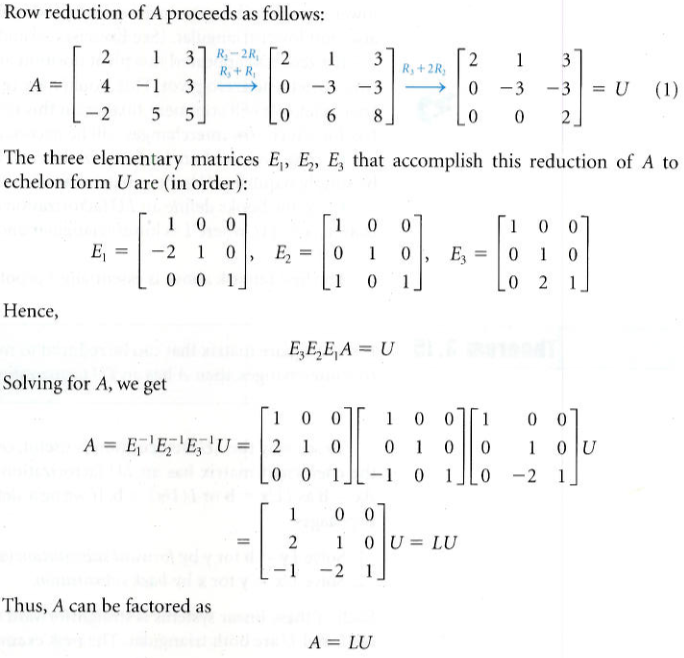
\includegraphics[scale = .5]{3}

NOTE: The row multipliers used in the preceding example are the entries of $L$ that are below its diagonal.

\subsection*{$P^TLU$ Factorization}
This method is an alternative form of the $LU$ factorization in which it handles row changes during Gaussian elimination. P is called the \textbf{permutation matrix}.\\*

Let $A$ be a square matrix. A factorization of $A$ as $A$ = $P^TLU$. This called a factorization of $A$.
\subsection*{Example}
Find a $P^TLU$ factorization of $A = \begin{bmatrix}
    0&0&6\\1&2&3\\2&1&4
\end{bmatrix}$.
\subsection*{Solution}
After reduing A to row echelon form, we get
$$\begin{bmatrix}
    1&2&3\\0&3&-2\\0&0&6
\end{bmatrix}$$

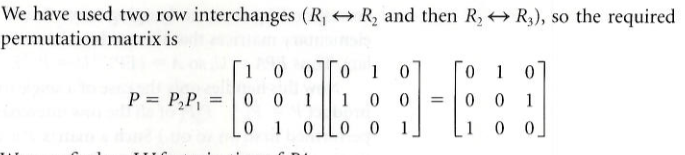
\includegraphics[scale = .5]{lu1}
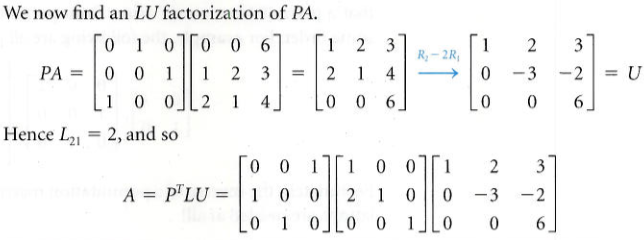
\includegraphics[scale = .5]{lu2}

\section{Subspaces, Basis, Dimension, and Rank}
\subsection*{Subspaces}
A \textbf{Subspace} of $\mathbb{R}^n$ is any collection $S$ of vectors in $\mathbb{R}^n$ such that
\begin{enumerate}
    \item The zero vector 0 in $S$.
    \item If $u$ and $v$ are in $S$, then $u+v$ is in $S$. (S is \textbf{\textit{closed under addition}}.)
    \item If $u$ is in $S$ and $c$ is a scalar, then $cu$ is in $S$. (S is \textbf{\textit{closed under scalar multiplication}}.)
\end{enumerate}
Let $v_1, v_2, \dots, v_k$ be vectors in $\mathbb{R}^n$. Then $span(v_1, v_2, \dots, v_k)$ is a subspace of $\mathbb{R}^n$.\\
Let $A$ be an $m\times n$ matrix. \begin{enumerate}
    \item The \textbf{row space} of $A$ is the subspace row(A) of $\mathbb{R}^n$ spanned by the rows of A. 
    \item The \textbf{column space} of $A$ is the subspace col(A) of $\mathbb{R}^n$ spanned by the columns of A. 
\end{enumerate}

\subsection*{Example}
Consider the matrix $A = \begin{bmatrix}
    1&-1\\0&1\\3&-3
\end{bmatrix}$. \\\begin{enumerate}[a]
    \item Determine whether $b = \begin{bmatrix}
        1\\2\\3
    \end{bmatrix}$ is the column space of $A$.
    \item Determine whether $w = \begin{bmatrix}
        4&5
    \end{bmatrix}$ is in the row space of $A$.
    \item Describe $row(A)$ and $col(A)$.
\end{enumerate}
\subsection*{Solution}
(a) We augment the matrix $[A|b]$ to determine if b is in col(A). After row reduction within the augmented matrix, 
$$\begin{bmatrix}
    1&0|&3\\0&1|&2\\0&0|0
\end{bmatrix}$$
Since the system is consistent, and has a unique solution, \textbf{b} is in $col(A)$.\\
(b) By solving the augmented matrix, $[\frac{A}{\textbf{w}}]$, and apply elementary row operations to reduce it to the form $\frac{A^\prime}{0}$, we have
$$\begin{bmatrix}
    1&0\\0&1\\0&0\\0&0
\end{bmatrix}$$ These calculations show that w is in $row(A)$.\\*
Let A be an $m\times n$ matrix. The \textbf{null space} of $A$ is the subspace of $\mathbb{R}^n$ consisting of solutions of the homogeneous linear system $Ax = 0$. It is denoted by $null(A)$.\\
\subsection*{Basis}
A \textbf{basis} for a subspace $S$ of $\mathbb{R}^n$ is a set of vectors in $S$ that \begin{enumerate}
    \item span S and 
    \item is linearly independent.
\end{enumerate}
\subsubsection*{Steps for finding the row, column, and the null spaces of a matrix A}
\begin{enumerate}
    \item Find the rref form $R$ of $A$.
    \item Use the nonzero row vectors of $R$ to form a basis for $row(A)$.
    \item Use the column vectors of $A$ that correspond to the columns of $R$ containing the leading 1s to form a basis for $col(A)$.
    \item Solve for the leading variables of $Rx = 0$ in terms of the free variables, set the free variables equal to parameters, substitute back into x, and write the result as a linear combination of \textit{f} vectors where f is the number of free variables. These f vectors form a basis for $null(A)$.
\end{enumerate}
\subsection*{Dimension and Rank}
\textbf{The Basis Theorem}\\
Let $S$ be a subspace of $\mathbb{R}^n$. Then any two bases for $S$ have the same number of vectors.\\* 

If $S$ is a subspace of $\mathbb{R}^n$, then the number of vectors in a basis for $S$ is called the \textbf{dimension} of $S$, denoted $dim S$.
Since the standard basis for $\mathbb{R}^n$ has $n$ vectors, $dim R^n = n$. 

The \textbf{rank} of a matrix $A$ is the dimension of its row and column spaces and is denoted by $rank(A)$.
The\textbf{nullity} of a matrix $A$ is the dimension of its null space and is denoted by $nullity(A)$.

\subsection*{Coordinates}
Let $S$ be a subspace of $\mathbb{R}^n$ and let $\beta = \{v_1, v_2, \dots, v_k\}$ be a basis for $S$. Let $v$ be a vector in $S$ and write $v = c_1v_1 + c_2v_2 + \dots + c_kv_k$. Then $c_1, c_2, \dots, c_k$ are called the \textbf{coordinates of v with respect to $\beta$} and the column vector
$$[v]_\beta = \begin{bmatrix}
    c_1\\c_2\\\vdots\\c_k
\end{bmatrix}$$
is called the \textbf{coordinate vector of v with respect to $\beta$}.
\subsection*{Example}
Let $\epsilon = \{e_1, e_2, e_3\}$ be the standard basis for $\mathbb{R}^3$. Find the coordinate vector of $v = \begin{bmatrix}
    2\\7\\4
\end{bmatrix}$\\ with respect to $\epsilon$.
\subsection*{Solution}
Since $v = 2e_1 + 7e_2 + 4e_3$, $$[v]_\epsilon = \begin{bmatrix}
    2\\7\\4
\end{bmatrix}$$

\section{Intro to Linear Transformations}
A \textbf{transformation} $T$ from $\mathbb{R}^n$ to $\mathbb{R}^m$ is a rule that assigns to each vector v in $\mathbb{R}^n$ a unique vector $T(v)$ in $\mathbb{R}^n$. 
\subsection*{Linear Transformations}
\begin{enumerate}
    \item $T(u+v) = T(u) + T(v)$
    \item $T(cv) = cT(v)$
\end{enumerate}
\textbf{Theorem}: Let $T: R^m\rightarrow R^n$ and $S: R^n\rightarrow R^p$ be linear transformations. Then $S\comp T: R^m\rightarrow R^p$ is a linear transformation. Moreover, their standard matricies related by\\
$[S\comp T] = [S][T]$
\textbf{Inverse Transformations}: Let $S$ and $T$ be linear transformations from $\mathbb{R}^n$ to $R_n$. Then S and T are inverse transformations if $S\comp T = I_n$ and $T\comp S = I_n$.
\setcounter{chapter}{3}
\chapter{Eigenvalues and Eigenvectors}

\section{Introduction to Eigenvalues and Eigenvectors}
Let $A$ be an $n\times n$ matrix. A scalar $\lambda$ is called an \textbf{eigenvalue} of $A$ if there is a nonzero vector x such that $Ax = \lambda x$. Such a vector x is called an \textbf{eigenvector} of $A$ corresponding to $\lambda$.

The \textbf{eigenspace} of $\lambda$ is denoted by $E_\lambda$ and is the collection of all eigenvectors corresponding to each other.

\subsection*{Example}
Show that $\lambda = 6$ is an eigenvalue of $A = \begin{bmatrix}
    7&1&-2\\-3&3&6\\2&2&2
\end{bmatrix}$ and find a basis for its eigenspace. 
\subsection*{Solution}
$A - 6I = \begin{bmatrix}
    1&1&-2\\-3&-3&7\\2&2&-4
\end{bmatrix}$\\ Row reduction produces $$\begin{bmatrix}
    1&1&-2\\0&0&0\\0&0&0
\end{bmatrix}$$ from which we can see that the null space of this is nonzero. Hence, 6 is an eigenvalue of $A$, and the eigenvectors corresponding to this eigenvalue satisfy $x_1+x_2-2x_3 = 0$. It follows that
$$E_6 = \{\begin{bmatrix}
    -x_2+2x_3\\x_2\\x_3
\end{bmatrix}\} = \{x_2\begin{bmatrix}
    -1\\1\\0
\end{bmatrix} + x_3\begin{bmatrix}
    2\\0\\1
\end{bmatrix}\} = span\{\begin{bmatrix}
    -1\\1\\0
\end{bmatrix}, \begin{bmatrix}
    2\\0\\1
\end{bmatrix}\}$$

\section{Determinants}
Let $A = \begin{bmatrix}
    a_{11}&a_{12}&a_{13}\\a_{21}&a_{22}&a_{23}\\a_{31}&a_{32}&a_{33}
\end{bmatrix}$. Then the \textbf{determinant} of $A$ is the scalar\\
$det A = |A| = a_{11}\begin{vmatrix}
    a_{22}&a_{23}\\a_{32}&a_{33}
\end{vmatrix} - a_{12}\begin{vmatrix}
    a_{21}&a_{23}\\a_{31}&a_{33}
\end{vmatrix} + a_{13}\begin{vmatrix}
    a_{21}&a_{22}\\a{31}&a_{32}
\end{vmatrix}$. This equation can also be wrote as 
$$\sum^3_{j=1} (-1)^{1+j}a_{1j}detA_{1j}$$

\subsection*{The Laplace Expansion Theorem}
The determinant of an $n\times n$ matrix $A$ = $a_{ij}$, where $n\geq 2$ can be computed as
$$det A = a_{i1}C_{i1}+\dots+a_{in}C_{in} \\= \sum^n_{i=1}a_{ij}C_{ij}$$
(which is the \textbf{cofactor expansion along the ith row}) and also as
$$det A = a_{1j}C_{1j}+\dots+a_{nj}C_{nk} \\= \sum^n_{j=1}a_{ij}C_{ij}$$
(the \textbf{cofactor expansion along the jth column})
\subsection*{Example}
Compute the determinant of the matrix
$$A = \begin{bmatrix}
    5&-3&2\\1&0&2\\2&-1&3
\end{bmatrix}$$ by (a) cofactor expansion along the third row and (b) cofactor expansion along the second column
\subsection*{Solution}
(a) We compute $$det A = a_{31}C_{31} + a_{32}C_{32} + a_{33}C_{33}$$
$$= 2\begin{vmatrix}
    -3&2\\0&2
\end{vmatrix} - (-1)\begin{vmatrix}
    5&2\\1&2
\end{vmatrix} + 3\begin{vmatrix}
    5&3\\1&0
\end{vmatrix} = 5$$
(b) In this case, we have 
$$det A = a_{12}C_{12} + a_{22}C_{22} + a_{32}C_{32}$$
$$= -(-3)\begin{vmatrix}
    1&2\\2&3
\end{vmatrix} + 0\begin{vmatrix}
    5&2\\2&3
\end{vmatrix} - (-1)\begin{vmatrix}
    5&2\\1&2
\end{vmatrix} = 5$$

\subsection*{Cramer's Rule and the Adjoint}
Let $A$ be an invertibel $n\times n $ matrix and let \textbf{b} be a vector in $R^n$. Then the unique solution \textbf{x} of the system Ax = b is given by
$$x_i = \frac{det(A_i(b))}{det A}\qquad for i = 1, \dots, n$$
\subsection*{Example}
Use Cramer's Rule to solve the system
$$x_1 + 2x_2 = 2$$ $$-x_1+4x_2 = 1$$
\subsection*{Solution}
We compute 
$$det A = \begin{vmatrix}
    1&2\\-1&4
\end{vmatrix} = 6,\qquad det(A_1(b)) = \begin{vmatrix}
    2&2\\1&4
\end{vmatrix} = 6, and \qquad det(A_2(b)) = \begin{vmatrix}
    1&2\\-1&1
\end{vmatrix} = 3$$ By Cramer's Rule,
$$x_1 = \frac{det(A_1(b))}{det A} = \frac{6}{6} = 1 and x_2 = \frac{det(A_2(b))}{det A} = \frac{3}{6} = \frac{1}{2}$$
The matrix $$[C_{ji}] = [C_{ij}]^T = \begin{bmatrix}
    C_{11}&C_{21}&\dots&C_{n1}\\
    C_{12}&C_{22}&\dots&C_{n2}\\
    \vdots&\vdots&\ddots&\vdots\\
    C_{1n}&C_{2n}&\dots&C_{nn}
\end{bmatrix}$$ is called the \textbf{adjoint} of A and is denoted by adj A. 

\section{Eigenvalues and Eigenvectors of $n\times n$ matricies}
The eigenvalues of a square matrix $A$ are precisely the solutions $\lambda$ of the equation
$$det(A-\lambda I) = 0$$
Let A be an $n\times n$ matrix.
\begin{enumerate}
    \item Compute the characteristic polynomial $det(A-\lambda I) of A$.
    \item Find the eigenvalues of $A$ by solving the characteristic equation $det(A-\lambda I) = 0 for \lambda$.
    \item For each eigenvalue $\lambda$, find the null space of the matrix $A-\lambda I$. This is the eigenspace $E_\lambda$, the nonzero vectors of which are the eigenvectors of $A$ corresponding to $\lambda$.
    \item Find a basis for each eigenspace.
\end{enumerate}
Refer back to Section 4.1 for an example.
\textbf{Theorem}: The eigenvalues of a triangular matrix are the entries on its main diagonal.

\section{Similarity and Diagonalization}
Let $A$ and $B$ be $n\times n$ matricies. We say that $A$ \textbf{is similar to} $B$ if there is an invertible $n\times n$ matrix $P$ such that $P^{-1}AP = B$. If $A$ is similar to $B$, we write $A\sim B$.\\

Let $A$ and $B$ be $n\times n$ matricies with $A\sim B$. Then
\begin{enumerate}[a]
    \item $det A = det B$
    \item $A$ is invertible if and only if $B$ is invertible
    \item $A$ and $B$ have the same rank.
    \item $A$ and $B$ have the same characteristic polynomial.
    \item $A$ and $B$ have the same eigenvalues.
\end{enumerate}
\subsection*{Example}
Let $A = \begin{bmatrix}
    1&2\\0&-1
\end{bmatrix}$ and $B = \begin{bmatrix}
    1&0\\-2&-1
\end{bmatrix}.$ 
\subsection*{Solution}
Then $A\sim B$, since 
$$\begin{bmatrix}
    1&2\\0&-1
\end{bmatrix}\begin{bmatrix}
    1&-1\\1&1
\end{bmatrix} = \begin{bmatrix}
    3&1\\-1&-1
\end{bmatrix} = \begin{bmatrix}
    1&-1\\1&1
\end{bmatrix}\begin{bmatrix}
    1&0\\-2&-1
\end{bmatrix}$$ Thus, $AP = PB$. 

\subsection*{Diagonalization}
An $n\times n$ matrix is $A$ is diagonalizable if there is a diagonal matrix $D$ such that $A$ is similar to $D$, that is, if there is an invertble matrix P such that $P^{-1}AP = D$.

\subsection*{Example}
Find if $A = \begin{bmatrix}
    1&3\\2&2
\end{bmatrix}$ is diagonalizable.
\subsection*{Solution}
$AP = PD$, From this, since $P = \begin{bmatrix}
    1&3\\1&-2
\end{bmatrix}$ and $D = \begin{bmatrix}
    4&0\\0&-1
\end{bmatrix}$, A is diagonalizable.
\textbf{The Diagonalization Theorem}
Let $A$ be an $n\times n$ matrix whose distinct eigenvalues are $\lambda_2, \dots, \lambda_k$. The following statements are equivalent.
\begin{enumerate}[a]
    \item $A$ is diagonalizable.
    \item The union $\beta$ of the bases of the eigenspaces of $A$ contains $n$ vectors.
    \item The algebraic multiplicity of each eigenvalue equals its geometric multiplicity.
\end{enumerate}

\subsection*{Gerschgorin's Disk Theorem}
Let $A = [a_{ij}]$ be a real or complex $n\times n$ matrix. Then every eigenvalue of $A$ is contained within a Gerschgorin disk.
Let $r_i$ denote the sum of the absolute values of the off-diagonal entries in the \textit{ith} row of $A$; that is, $r_i = \sum_{j\neq i}|a_{ij}|$. The \textbf{ith Gerschgorin disk} is the circular disk $D_i$ in the complex plane with center $a_{ii}$ and radius $r_i$. That is,
$$D_i = \{z in \mathfrak{C}:|z-a_{ii}| \leq r_i\}$$

\subsection*{Example}
Sketch the Gerschgorin disks and the eigenvalues for the following matrix. $$A = \begin{bmatrix}
    2&1\\2&-3
\end{bmatrix}$$
\subsection*{Solution}
The Gerschgorin disk is centered at 2 with radii 1. The characteristic polynomial of $A$ is $\lambda^2+\lambda - 8$

\subsection*{The Perron-Frobenius Theorem}
Let $A$ be an irreducible nonnegative $n\times n$ matrix. Then A has a real eigenvalue $\lambda$ with the following properties:
\begin{enumerate}[a]
    \item $\lambda_1 > 0$
    \item $\lambda_1$ has a corresponding positive eigenvector.
    \item $\lambda$ has any other eigenvalue of $A$, then $|\lambda| \leq \lambda_1$. If A is primitive, then this inequality is strict. 
    \item $\lambda$ is an eigenvalue of A such that $|\lambda| = \lambda_1$, then $\lambda$ is a complex root of the equation$\lambda^n = \lambda^n_1 = 0$
    \item $\lambda_1$ has algebraic multiplicity 1.
\end{enumerate}





\setcounter{chapter}{4}
\chapter{Continuous Random Variables}
\section{Introduction}
\begin{definition}[Continuous Random Variables]
Random variables who set of possible values are countably infinite. 
\end{definition}
The \textbf{probability density function} can be defined as \[P\{X\in B\} = \int_B f(x) dx\]
The \textbf{cumulative density function} has a continuous relationship defined with the PDF. 
\[P\{X < a\} = P\{X\leq a\} = F(a) = \int^a_{-\infty} f(x) dx\]
\subsection*{Example}
The amount of time in hours that a computer functions before breaking down is a continouous random variable with probabiltiy density function given by 
\begin{equation*}
f(x) 
\left\{
    \begin{array}{lr}
        \lambda e^{-x/100} x\geq 0\\
        0 x < 0
    \end{array}
\right\}
\end{equation*}
What is the probability that 
\begin{enumerate}[a. ]
    \item a computer will function between 50 and 150 hours before breaking down?
    \item it will function for fewer than 100 hours?
\end{enumerate}
\subsubsection*{Solution}
Since \[1 = \int^\infty_{-\infty} f(x) dx = \lambda\int^\infty_0 e^{-x/100} dx\]
we have \[1 = -\lambda(100)e^{-x/100}\big|^\infty_0 = 100\lambda\text{ or } \lambda = \frac{1}{100}\]
Then the probability that a computer will function between 50 and 150 hours before breaking down is given by 
\[P\{50 > x > 150\} = \int^150_50 \frac{1}{100}e^{-x/100} dx = -e^{-x/100}\big|^150_50\]
\[=e^{-1/2} - e^{-3/2}\approx .383\]
Similarily, 
\[P\{X < 100\} = \int^100_0 \frac{1}{100}e^{-x/100} dx = -e^{-x/100}\big|^100_0 = 1 - e^{-1}\approx .632\]
$63.2\%$ of the time a computer will fail before registering 100 hours of use. 
\section{Expectation and Variance of Continuous Random Variables}
Suppose $X$ is a continuous random variable. Then the expected value of $X$ is defined by 
\[E[X] = \int^\infty_{-\infty} xf(x) dx\]
\subsection*{Example}
The density function of $X$ is given by
\begin{equation*}
f(x) =
\left\{
    \begin{array}{lr}
        1 \text{ if } 0\leq x\leq 1\\
        0 \text{ otherwise}
    \end{array}
\right\}
\end{equation*}
Find $E[e^X]$. \\
Let $Y = e^X$. We start by determining $F_Y$, the CDF of $Y$. For $1\leq x\leq e$,
\begin{equation*}
    \begin{split}
        F_Y(x) &= P\{Y\leq x\}\\
        &= P\{e^x\leq x\}\\
        &= P{X\leq log(x)}\\
        &= \int^{log(x)}_0 f(y) dy\\
        &= log(x)
    \end{split}
\end{equation*}
By differentiating $F_Y(x)$ we can say that the PDF of $Y$ is given by \[f_Y(x) = \frac{1}{x}\qquad 1\leq x\leq e\]
Then, 
\begin{equation*}
    \begin{split}
        E[e^x] = E[Y] &= \int^\infty_{-\infty} xf_Y(x) dx\\
        &= \int^e_1 dx\\
        &= \boxed{e - 1}
    \end{split}
\end{equation*}
\begin{lemma}
For a nonnegative random variable $Y$, \[E[Y] = \int^\infty_0 P\{Y > y\} dy\]
\end{lemma}
\begin{corollary}
If a and b are constants, then \[E[aX+b] = aE[X] + b\]
\end{corollary}
\section{Uniform Random Variable}
\begin{definition}[Uniform Random Variable]
    A random variable is said to be \textbf{uniformly distributed} over the interal $(\alpha,\beta)$ if its probability density function is given by 
    \begin{equation*}
        f(x) =
        \left\{
            \begin{array}{lr}
                \frac{1}{\beta - \alpha} \text{ if } 0 < x < 1\\
                0 \text{ otherwise}
            \end{array}
        \right\}
    \end{equation*}
\end{definition}
To find the variance and expected value of the uniform random variable, we have 
\begin{equation*}
    \begin{split}
        E[X] &= \int^\infty_{-\infty} xf(x) dx\\
        &= \int^\beta_\alpha \frac{x}{\beta - \alpha} dx\\
        &= \frac{\beta^2 - \alpha^2}{2(\beta - \alpha)}\\
        &= \frac{\beta + \alpha}{2}
    \end{split}
\end{equation*}
In other words, the expected value is the midpoint of that interval. 
For the variance, we calculate $E[X^2]$ first. 
\begin{equation*}
    \begin{split}
        E[X^2] &= \int^\beta_\alpha \frac{1}{\beta - \alpha}x^2 dx\\
        &= \frac{\beta^3 - \alpha^3}{3(\beta - \alpha)}\\
        &= \frac{\beta^2 + \alpha\beta + \alpha^2}{3}
    \end{split}
\end{equation*}
So, we have 
\begin{equation*}
    \begin{split}
        Var(X) &= \frac{\beta^2 + \alpha\beta + \alpha^2}{3} - \frac{(\alpha + \beta)^2}{4}\\
        &= \frac{(\beta - \alpha)^2}{12}
    \end{split}
\end{equation*}
\subsection*{Example}
Buses arrive at a specified stop at 15-minute intervals starting at 7. That is,
they arrive at 7, 7:15, 7:30, 7:45, and so on. If a passenger arrives at the stop at
a time that is uniformly distributed between 7 and 7:30, find the probability that he
waits
\begin{enumerate}[a. ]
    \item less than 5 minutes for a bus;
    \item more than 10 minutes for a bus. 
\end{enumerate}
\subsubsection*{Solution}
Let $X$ denote the number of minutes past 7 that the passenger arrives at the stop.
Since $X$ is a uniform random variable over the interval (0, 30), it follows that the
passenger will have to wait less than 5 minutes if (and only if) he arrives between
7:10 and 7:15 or between 7:25 and 7:30. Hence, the desired probability for part
(a) is \[P\{10 < X < 15\} + P\{25 < X < 30\} = \int^15_10 \frac{1}{30} dx + \int^30_25 \frac{1}{30} dx = \frac{1}{3}\]
Similarly, he would have to wait more than 10 minutes if he arrives between 7
and 7:05 or between 7:15 and 7:20, so the probability for part (b) is 
\[P\{0 < X < 5\} + P\{15 < X < 20\} = \frac{1}{3}\]
\section{Normal Random Variable}
\begin{definition}[Normal Random Variable]
    We say that $X$ is a normally distributed r.v. with parameters $\mu$ and $\sigma^2$ if the density of $X$ is given by
    \[f(x) = \frac{1}{\sqrt{2\pi}\sigma}e^{-(x-\mu)^2/2\sigma^2}\]
    The density function is a bell shaped curve that is symmetric about $\mu$. The expected value is 0 with variance 1. 
\end{definition}
An important fact about normal random variables is that if $X$ is normally distributed with parameters $\mu$ and $\sigma^2$, then $Y = aX + b$ is normally distributed with parameters $a\mu + b$ and $a^2\sigma^2$.\\
The cumulative distribution function is often represented by $\phi(x)$
\[\phi(x) - \frac{1}{\sqrt{2\pi}}\int^x_{-\infty} e^{-y^2/2} dy\]
\begin{theorem}[The DeMoivre - Laplace Limit Theorem]
If $S_n$ denotes the number of successes that occur when $n$ independent trials each resulting in a success with probability $p$, are performed, then, for any $a < b$, \[P\{a\leq \frac{S_n - np}{\sqrt{np(1-p)}}\leq b\}\rightarrow \phi(b) - \phi(a)\]
as $n\rightarrow\infty$.
\end{theorem}
When $n$ is large, a binomial random variable with parameters n and p will have approximately the same distribution as a normal random variable with the same mean and variance as the binomial. 
\section{Exponential Random Variables}
\begin{definition}[Exponential Random Variables]
    A continuous random variable whose probability density function is given for some $\lambda > 0$ by
    \begin{equation*}
        f(x) =
        \left\{
            \begin{array}{lr}
                \lambda e^{-\lambda x} \text{ if } x\geq 0\\
                0 \text{ if } x < 0
            \end{array}
        \right\}
    \end{equation*}
    is said to be an \textbf{exponential} random variable. The CDF $F(a)$ is given by \[1- e^{-\lambda a}\, a\geq 0\]. The expected value and variance are \[E[X] = \frac{1}{\lambda}\qquad Var(X) = \frac{1}{\lambda^2}\]
\end{definition}
\section{Gamma Distribution}
A random variable is said to have a gamma distribution with parameters $(\alpha, \lambda), \lambda > 0, \alpha > 0$ if its density function is given by 
\begin{equation*}
    f(x) =
    \left\{
        \begin{array}{lr}
            \frac{\lambda e^{-\lambda x}(\lambda x)^{\alpha -1}}{\Gamma(\alpha)}\qquad x\geq 0\\
            0 \qquad x < 0
        \end{array}
    \right\}
\end{equation*}
where $\Gamma (\alpha)$, the \textit{gamma function} is defined as \[\Gamma(\alpha) = \int^\infty_0 e^{-y}y^{\alpha-1} dy\]
It follows that the density function is \[f(t) = \frac{\lambda e^{-\lambda t}(\lambda t)^{n-1}}{(n-1)!}\] and the expected value with variance is given as \[E[X] = \frac{\alpha}{\lambda}\qquad Var(X) = \frac{\alpha}{\lambda^2}\]

\section{The Distribution of a Function of a Random Variable}
Often, we know the probability distribution of a random variable and are interested in determining the distribution of some function of it. For instance, suppose that we know the distribution of $X$ and want to find the distribution of $g(X)$. We then need to express the event that $g(X)\leq y$ in terms of $X$ being a set. 
\begin{theorem}
    Let $X$ be a continuous random variable having probability density function $f_x$. Suppose that $g(x)$ is stricitly monotonic, differentiable function of $x$. Then the random variable $Y$ defined by $Y = g(X)$ has a probability density function given by 
    \begin{equation*}
        f_Y(y) =
        \left\{
            \begin{array}{lr}
                f_X[g^{-1}(y)]\left|\frac{d}{dy}g^{-1}(y)\right| \, \text{ if } y = g(x) \text{ for some } x\\
                0 \text{ if } y\neq g(x) \text{ for all } x
            \end{array}
        \right\}
    \end{equation*}
    wehre $g^{-1}(y)$ is defined to equal the value of x such that $g(x) = y$.
\end{theorem}
\subsection*{Example}
Let $X$ be a continuous nonnegative random variable with density function $f$, and let $Y = X^n$. Find $f_Y$, the probability density function of $Y$.
\subsubsection*{Solution}
if $g(x) = x^n$, then \[g^{-1}(y) = y^{1/n}\] and \[\frac{d}{dy}\{g^{-1})(y)\} = \frac{1}{n}y^{1/n-1}\]
We obtain for $y\geq 0$ \[f_Y(y) = \frac{1}{n}y^{1/n-1}f(y^{1/n})\]
\subsection*{The Lognormal Distribution}
If $X$ is a normal random variable with mean $\mu$ and variance $\sigma^2$, then the random variable \[Y = e^x\] is said to be a \textit{lognormal} random variable with parameters $\mu$ and $\sigma^2$. The lognormal is often used as the distribution of the ratio of a price of a security at the end of one day to its price at the end of the prior day.  That is, if $S_n$ is the price of some security at the end of the day $n$, then it is often supposed that $\frac{S_n}{S_n - 1}$ is normal. Thus, to assume that fraction is lognormal is to assume that \[S_n = S_{n-1}e^x\] where $X$ is normal. 
\setcounter{chapter}{5}
\chapter{Vector Spaces}

\section{Vector Spaces and Subspaces}
Let $V$ be a set on two operations, called addition and scalar multiplication, have been defined. The \textit{sum} is defined by $u+v$. The scalar multiple of $\textbf{u}$ is defined by c.\\
If the following axioms hold for all $u$, $v$, and $w$ in \textit{V} and for all scalars c and d, then V is called a \textbf{vector space} and its elements are called vectors.
\begin{enumerate}
    \item $u+v$ is in \textit{V}.
    \item $u+v = v+u$
    \item $(u+v)+w = u + (v+w)$
    \item There exists an element \textbf{0} in \textit{V}, called a \textbf{zero vector}, such that \textbf{$u+0 = u$}.
    \item For each \textbf{u} in \textit{V}, there is an element \textbf{-u} in \textit{V} such that \textbf{u + (-u) = 0}.
    \item c\textbf{u} is in \textit{V}.
    \item $c(u+v) = cu + cv$
    \item $(c+d)u = cu + du$
    \item c(du) = (cd)u
    \item 1u = u
\end{enumerate}
\subsection*{Properties of Vector Spaces}
Let \textit{V} be a vector space, \textbf{u} a vector in \textit{V}, and \textit{c} a scalar.
\begin{enumerate}
    \item 0u = 0
    \item c0 = 0
    \item (-1)u = -u
    \item If cu = 0, then c = 0 or u = 0
\end{enumerate}
\subsection*{Example}
Show that the set $W$ of all vectors of the form $$\begin{bmatrix}
    a\\b\\-b\\a
\end{bmatrix}$$ is a subspace of $\mathbb{R}^4$.
\subsection*{Solution}
Let $u$ and $v$ be in W
$$v = \begin{bmatrix}
    c\\d\\-d\\c
\end{bmatrix}$$ Then
$$u + v = \begin{bmatrix}
    a+c\\b+d\\-(b+d)\\a+c
\end{bmatrix}$$
so u + v is also in W because it has the right form. Similarly, if k is a scalar, then $$ku = \begin{bmatrix}
    ka\\kb\\-kb\\ka
\end{bmatrix}$$ so k\textbf{u} is in $W$.\\
Since W is closed under vector addition and scalar multiplication, W is a subspace of $\mathbb{R}^4$.

\section{Linear Independece, Basis, and Dimension}
A set of vectors ${v_1, v_2, \dots, v_k}$ in a vector space $V$ is \textbf{linearly dependent} if there are scalars $c_1, c_2, \dots, c_k$ at least one of which is not zero, such that
$$c_1v_1 + c_2v_2 + \dots + c_kv_k = 0$$
A set of vectors that is not linearly dependent is said to be \textbf{linearly independent}.\\*

A set of vectors ${v_1, v_2, \dots, v_k}$ in a vector space $V$ is linearly dependent if and only if at least one of the vectors can be expressed as a linear combination of the others.

\subsection*{Example}
In $\mathfrak{P}^2$, determine whether the set $\{1+x, x+x^2, 1+x^2\}$ is linearly independent.

\subsection*{Solution}
Let $c_1$, $c_2$, and $c_3$ be scalars such that
$$c_1(1+x)+c_2(x+x^2)+c_3(1+x^2) = 0$$
Then $$(c_1 + c_3) + (c_1 + c_2)x + (c_2 + c_3)x^2 = 0$$
This implies that $$c_1 +\qquad c_3 = 0$$ $$c_1 + c_2\qquad = 0$$ $$\qquad c_2 + c_3 = 0$$
the solution to which $c_1 = c_2 = c_3 = 0$. It follows that $\{1+x, x+x^2, 1+x^2\}$ is linearly independent.

\subsection*{Basis}
A subset $\beta$ of a vector space $V$ is a \textbf{basis} for $V$ if 
\begin{enumerate}
    \item $\beta spans V$ and 
    \item $\beta$ is linearly independent.
\end{enumerate}
If \textbf{$e_i$} is the \textit{i}th column of the $n\times n$ identity matrix, then $\{e_1, e_2, \dots, e_n\}$ is a basis for $\mathbb{R}^n$ called the \textbf{standard basis}.

\subsection*{Coordinates}
For every vector $v$ in $V$, there is exactly one way to write $v$ as a linear combination of the basis vectors in $\beta$.
Let $\beta$ = ${v_1, v_2, \dots, v_n}$ be a basis for a vector space $V$. Let \textbf{v} be a vector in $V$. Then $c_1, c_2, \dots, c_n$ are called the \textbf{coordinates of v with respect to $\beta$} and the column vector\\
$$[v]_B = \begin{bmatrix}
    c_1\\c_2\\\vdots\\c_n
\end{bmatrix}$$ is called the \textbf{coordinate vector of v with respect to $\beta$}.

\subsection*{Dimension}
Let $\beta = \{v_1, v_2,\dots, v_n\}$ ne a nasis for a vector space $V$.
\begin{enumerate}
    \item Any set of more than \textit{n} vectors in $V$ must be linearly dependent.
    \item Any set of fewer than \textit{n} vectors in $V$ cannot span $V$.
\end{enumerate}
\textbf{The Basis Theorem}: If a vector space $V$ has a basis with \textit{n} vectors, then every basis for $V$ has exactly \textit{n} vectors.\\*

A vector space $V$ is called \textbf{finite-dimensional} if it has a basis consitting of finitely many vectors. The \textbf{dimension} of V, denoted by dim $V$, si the number of vectors in a basis for V. The deimension of the zaero vector space is defined to be zero. A vector space that has no finite basis is called \textbf{infite-dimensional}.

Let $V$ be a vector space with $dim V = n$. Then
\begin{enumerate}[a]
    \item Any linearly independent set in $V4$ contains at most \textit{n} vectors.
    \item Any spanning set for $V$ contains at least \textit{n} vectors.
    \item Any linearly independent set of exactly \textit{n} vectors in $V$ is a basis for $V$. 
    \item Any spanning set for $V$ consiting of exactly \textit{n} vectors is a basis for $V$.
    \item Any linearly independent set in $V$ can be extended for a basis in $V$.
    \item Any spanning set for $V$ can be reduced to a basis for $V$.
\end{enumerate}

\section*{Change of Basis}
Let $\beta$ = $\{u_1, \dots, u_n\}$ and $C = \{v_1, \dots, v_n\}$ be bases for a vector space $V$. The $n\times n$ matrix whose columns are the coordinate vectors $[u_1]_C, \dots, [u_n]_C$ of the vectors in $\beta$ with respect to $C$ is denoted by\\ $P_{C\leftarrow \beta}$.\\
Think of $\beta$ as the "old basis" and $C$ as the "new basis".

Let $\beta$ = $\{u_1, \dots, u_n\}$ and $C = \{v_1, \dots, v_n\}$ be bases for a vector space $V$ and let $P_{C\leftarrow \beta}$ be the change-of-basis matrix from $\beta$ to $C$. Then
\begin{enumerate}[a]
    \item $P_{C\leftarrow \beta}[x]_\beta = [x]_C for all x in V$.
    \item $P_{C\leftarrow \beta}$ is the unique matrix $P$ with the property that $P[x]_\beta = [x]_C for all x in V$
    \item P is invertible and $(P_{C\leftarrow \beta})^{-1} = P_{\beta \leftarrow C}$
\end{enumerate}
\subsection*{Example}
Find the change of basis matricies $P_{C\leftarrow \beta}$ and $P_{\beta \leftarrow C}$ for the bases $\beta = \{1, x, x^2\}$ and $C = \{1+x, x+x^2, 1+x^2\}$ of $\mathfrak{P}_2$. Then find the coordinate vector of $p(x) = 1+2x-x^2$ with respect to $C$.
\subsection*{Solution}
$[1+x]_\beta = \begin{bmatrix}
    1\\1\\0
\end{bmatrix}\qquad [x+x^2]_\beta = \begin{bmatrix}
    0\\1\\1
\end{bmatrix}\qquad [1+x^2]_\beta = \begin{bmatrix}
    1\\0\\1
\end{bmatrix}\qquad P_{\beta \leftarrow C} = \begin{bmatrix}
    1&0&1\\1&1&0\\0&1&1
\end{bmatrix}$\\*
$P_{C\leftarrow \beta} = (P_{\beta \leftarrow C})^{-1} = \begin{bmatrix}
    \frac{1}{2}&\frac{1}{2}&\frac{-1}{2}\\\frac{-1}{2}&\frac{1}{2}&\frac{1}{2}\\\frac{1}{2}&\frac{-1}{2}&\frac{1}{2}
\end{bmatrix}$\\*
$[p(x)]_C = P_{C\leftarrow \beta}[p(x)]_\beta = \begin{bmatrix}
    \frac{1}{2}&\frac{1}{2}&\frac{-1}{2}\\\frac{-1}{2}&\frac{1}{2}&\frac{1}{2}\\\frac{1}{2}&\frac{-1}{2}&\frac{1}{2}
\end{bmatrix}\begin{bmatrix}
    1\\2\\-1
\end{bmatrix} = \begin{bmatrix}
    2\\0\\-1
\end{bmatrix}$\\
\subsection{The Gauss-Jordan Method for Computing a Change-of-Basis Matrix}
Let $\beta$ = $\{u_1, \dots, u_n\}$ and $C = \{v_1, \dots, v_n\}$ be bases for the vector space V. Now let $\beta$ = $\{[u_1]_E, \dots, [u_n]_E\}$ and $C = \{[v_1]_E, \dots, [v_n]_E\}$. Then row reduction applied to the $n\times 2n$ augmented matrix [C|B] produces
$$[C|\beta] = [I|P_{C\leftarrow \beta}]$$
\subsection*{Example}
In $M_22$, let $B$ be the basis$\{E_{11}, E_{21}, E_{12}, E_{22}\}$ and let $C$ be the basis, where $\{A, B, C, D\}$
Find the change-of-basis matrix $P_{C\leftarrow \beta}$ and verify that $[X]_C = P_{C\leftarrow \beta}[X]_\beta$ for $X = \begin{bmatrix}
    1&2\\3&4
\end{bmatrix}$
\subsection*{Solution}
$B = P_{\epsilon\leftarrow B} = \begin{bmatrix}
    1&0&0&0\\0&0&1&0\\0&1&0&0\\0&0&0&1
\end{bmatrix}$ and $C = P_{\epsilon\leftarrow C} = \begin{bmatrix}
    1&1&1&1\\0&1&1&1\\0&0&1&1\\0&0&0&1
\end{bmatrix}$
Row reduction produces \\$P_{C\leftarrow \beta} = \begin{bmatrix}
    1&0&-1&0\\0&-1&1&0\\0&1&0&-1\\0&0&0&1m
\end{bmatrix}$

\section{Linear Transformations}
A \textbf{linear transformation} from a vector space $V$ to a vector space $W$ is a mapping $T: V\rightarrow W$ such that, for all $u$ and $v$ in $V$ and for all scalars c,\\
\begin{enumerate}
    \item $T(u+v) = T(u) + T(v)$
    \item $T(cu) = cT(u)$
\end{enumerate}
$T: V\rightarrow W$ is a linear transformation if any only if $T(c_1v_1 + c_2v_2 +\dots+ c_kv_k) = c_1T(v_1) + c_2T(v_2) +\dots + c_kT(v_k)$.
\subsection*{Example}
Define $T: M_{nn}\rightarrow M_{nn} by T(A) = A^T.$ Show that $T$ is a linear transformation.
\subsection*{Solution}
We check that, for $A$ and $B$ in $M_{nn}$ and scalars c.
$$T(A+B) = (A+B)^T = A^T + B^T = T(A) + T(B)$$and \qquad $$T(cA) = (cA)^T = cA^T = cT(A)$$ Therefore, $T$ is a linear transformation.\\
Let $T: V\rightarrow W$ be a linear transformation. Then, \begin{enumerate}
    \item $T(0) = 0$
    \item $T(-v) = -T(v)$
    \item $T(u-v) = T(u) - T(v)$
\end{enumerate}
\subsection*{Composition of Linear Transformations}
If $T: U\rightarrow V$ and $S: V\rightarrow W$ are linear transformations, then the \textbf{composition of S with T} is the mapping $S\comp T$, defined by 
$$(S\comp T)(u) = S(T(u))$$
where u is in $U$.
\subsection*{Inverses of Linear Transformations}
A linear transformation $T: W\rightarrow V$ is invertible if there is a linear transformation $T^\prime: V\rightarrow W$ such that
$$T^\prime\comp T = I_V$$ and $$T\comp T^\prime = I_W$$ In this case, $T^\prime is called an inverse for T$

\section{Kernel and Range of a Linear Transformation}
The \textbf{kernel} of $T$, denoted $ker(T)$, is the set of all vectors in $V$ that are mapped by $T$ to 0 in $W$. That is,
$$ker(T) = \{v in V: T(v) = 0\}$$
The \textbf{range} of $T$, denoted $range(T)$, is the set of all vectors in $W$ that are images of vectors in $V$ under $T$. That is, \\
$range(T) = \{T(v) : v in V\} \\=\{win W: w = T(v) for some v in V\}$\\

\subsection*{Example}
Find the kernel and range of the differential operator $D: \mathfrak{P}_3\rightarrow\mathfrak{P}_2$ defined by $D(p(x)) = p^\prime(x)$.
\subsection*{Solution}
$$ker(D) = \{a+bx+cx^2+dx^3:D(a+bx+cx^2+dx^3) = 0\}$$
$$\{a+bx+cx^2+dx^3 : b+2cx+3dx^2 = 0\}$$ $$\{a+bx+cx^2+dx^3 : b = c = d =0\}$$ $$= \{a : a in \mathfrak{R}\}$$
$range(D)$ in all polynomials in $P_2$
\subsection*{Rank and Nullity}
The \textbf{rank} of $T$ is the dimension of range of T and is denoted by rank(T). The \textbf{nullity} of $T$ is dimension of the kernel of T and is denoted by nullity(T).
\subsection*{Example}
Find the rank and the nullity of the linear transformation $D: \mathfrak{P}_3\rightarrow\mathfrak{P}_2$ defined by $D(p(x)) = p^\prime(x)$.
\subsection*{Solution}
rank(D) = dim $\mathfrak{P}_2 = 3$\\
nullity(D) = dim(ker(D)) = 1\\
Let $T: V\rightarrow W$ be a linear transformation from a finite-dimensional vector space $V$ into a vector space $W$. Then
$$rank(T) + nullity (T) = dim V$$
\subsection*{One-to-One and Onto Linear Transformations}
A linear transformation $T:V\rightarrow W$ is called \textbf{one-to-one} if T maps distinct vectors in $V$ to distinct vectors in $W$. If range(T) = $W$, then T is called \textbf{onto}.
\begin{enumerate}[a]
    \item $T:V\rightarrow W$ is one-to-one of, for all $u$ and $v$ in $V$, $u\neq v$ implies that $T(u)\neq T(v)$.
    \item $T:V\rightarrow W$ is one-to-one of, for all $u$ and $v$ in $V$, $T(u) =  T(v)$ implies that $u=v$.
    \item $T:V\rightarrow W$ is onto if, for all $u$ and $v$ in $V$, there is at least one $v$ in $V$ such that $w = T(v)$
\end{enumerate}
A linear transformation $T:V\rightarrow W$ is one-to-one if and only if $ker(T) = \{0\}$. 

Let $dim V = dim W = n$. Then a linear transformation $T:V\rightarrow W$ is one-to-one if and only if it is onto.

\subsection*{Isomorphisms of Vector Spaces}
A linear transformation $T:V\rightarrow W$ is called an \textbf{isomorphism} if it is one-to-one and onto. If $V$ and $W$ are two vector spaces such that there is an isomorphism from $V$ to $W$, then we say $V$ is \textbf{isomorphic} to $W$ and write $V = W$.
\subsection*{Example}
Let $W$ be the vector space of all symmetric $2\times 2$ matricies. Show that $W$ is isomorphic to $\mathbb{R}^3$.
\subsection*{Solution}
W is represented by the form $\begin{bmatrix}
    a&b\\b&c
\end{bmatrix}$, so $dim W = 3$.

\section*{The Matrix of a Linear Transformation}
Let $V$ and $W$ be two finite-dimensional vector spacfes with bases B and C, respectively, where B = $\{v_1, \dots, v_n\}$. 
If $T:V\rightarrow W$ is a linear transformation, then the $m\times n$ matrix $A$ defined by\\
$A = [T(v_1)_C][T(v_2)_C]\dots[T(v_n)_C$

\subsection*{Example}
Let $T: R^3 \rightarrow R^n$ be the linear transformation defined by
$$T\begin{bmatrix}
    x\\y\\z
\end{bmatrix} = \begin{bmatrix}
    x-2y\\x+y-3z
\end{bmatrix}$$ and let $B = \{e_1, e_2, e_3\}$ and $C = \{e_2, e_1\}$ be bases for $R_3$ and $R_2$, respectively. Find the matrix of $T$ with respect to $B$ and $C$.
\subsection*{Solution}
$$T(e_1) = T\begin{bmatrix}
    1\\0\\0
\end{bmatrix} = \begin{bmatrix}
    1\\1
\end{bmatrix}, \qquad T(e_2) = T\begin{bmatrix}
    0\\1\\0
\end{bmatrix} = \begin{bmatrix}
    -2\\1
\end{bmatrix}, \qquad T(e_3) = T\begin{bmatrix}
    0\\0\\1
\end{bmatrix} = \begin{bmatrix}
    0\\-3
\end{bmatrix}$$

$$e_2+e_1 = a\begin{bmatrix}
    0\\1
\end{bmatrix} + b\begin{bmatrix}
    1\\0
\end{bmatrix} = \begin{bmatrix}
    1\\1
\end{bmatrix}\qquad [T(e_1)]_C = \begin{bmatrix}
    1\\1
\end{bmatrix}$$

$$e_2+e_1 = a\begin{bmatrix}
    0\\1
\end{bmatrix} + b\begin{bmatrix}
    1\\0
\end{bmatrix} = \begin{bmatrix}
    -2\\1
\end{bmatrix}\qquad [T(e_2)]_C = \begin{bmatrix}
    1\\-2
\end{bmatrix}$$

$$e_3 + e_1 = a\begin{bmatrix}
    0\\1
\end{bmatrix} + b\begin{bmatrix}
    1\\0
\end{bmatrix} = \begin{bmatrix}
    0\\-3
\end{bmatrix}\qquad [T(e_2)]_C = \begin{bmatrix}
    -3\\0
\end{bmatrix}$$

$$A = [T(e_1)]_C[T(e_2)]_C[T(e_3)]_C = \begin{bmatrix}
    1&1&-3\\1&-2&0
\end{bmatrix}$$
$$A[v]_B = [T(v)]_C\qquad v_B = \begin{bmatrix}
    1\\3\\-2
\end{bmatrix}$$
$$[T(v)]_C = \begin{bmatrix}
    -5\\10
\end{bmatrix}_C = \begin{bmatrix}
    10\\-5
\end{bmatrix}$$
$$\begin{bmatrix}
    1&1&-3\\1&-2&0
\end{bmatrix}\begin{bmatrix}
    1\\3\\-2
\end{bmatrix} = \begin{bmatrix}
    10\\-5
\end{bmatrix}$$

\subsection*{Matricies of Composite and Inverse Linear Transformations}
Let $U$, $V$, and $W$ be finite-dimensional vector spaces with bases B, C, and D, respectively. A linear transformation $T:U\rightarrow V$ and $S:V\rightarrow W$ be linear transformation. Then
$$[S\comp T]_{D\leftarrow B} = [S]_{D\leftarrow C}[T]_{C\leftarrow B}$$

\subsection*{Example}
The linear transformation $T: R^2 \rightarrow \mathfrak{P}_1$ defined by $T\begin{bmatrix}
    a\\b
\end{bmatrix} = a+ (a+b)x$ were shown to be one to one and onto and hence invertible. Find $T^-1$.

\section{Applications}
\subsection*{Homogeneous Libear Differential Equations}
Let S be the solution space of $y^{\prime\prime} + ay^\prime + by = 0$\\
and let $\lambda_1$ and $\Lambda_2$ be the roots of the characteristic equation $\lambda^2 + a\lambda + b = 0$
\begin{enumerate}[a]
    \item If $\lambda_1\neq\lambda_2$, then $\{e^{\lambda_1t}, e^{\lambda_2}t\}$ is a basis for S. 
    \item If $\lambda_1\neq\lambda_2$, then $\{e^{\lambda_1t}, te^{\lambda_1}t\}$ is a basis for S.
\end{enumerate}
Therefore, the solutions are $$y = c_1e^{\lambda_1t} + c_2e^{\lambda_2t} and y = c_1e^{\lambda_1t} + c_2te^{\lambda_1t}$$
\subsection*{Example}
Find all solutions of $$y^{\prime\prime} - 5y^\prime + 6y = 0$$
\subsection*{Solution}
Make the Equation in terms of lambda.
$$y^{\prime\prime} - 5y^\prime + 6y = 0\rightarrow\lambda^2 + 5\lambda + 6 = 0$$
$$(\lambda - 2)(\lambda - 3)= 0\qquad \lambda = 2,3$$
Basis is $\{e^{2t}, e^{3t}\}\qquad y = c_1e^{2t} + c_2e^{3t}$
\setcounter{chapter}{6}
\chapter{Properties of Expectation}
\section{Review}
For discrete, \[E[X] = \sum_x xp(x)\]. For continuous, \[E[X] = \int^\infty_{\infty} xf(X) dx\]
Since $E[X$ is a weighted average of the possibole values of $X$, it follows that if $X$ must lie between $a$ and $b$, then so must its expected value. That is, if \[P\{a\leq X\leq b\} = 1\] then \[a\leq E[X]\leq b\]
\section{Expectation of Sums of Random Variables}
If $X$ and $Y$ have a joint probability mass function $p(x,y)$, then \[E[g(X,Y) = \sum_y\sum_x g(x,y)p(x,y)\]
If $X$ and $Y$ have a joint probability density function $f(x,y)$, then \[E[g(X,Y) = \int^\infty_{-\infty} \int^\infty_{-\infty} g(x,y)f(x,y) dx dy\]
\subsection*{Example}
An accident occurs at a point that is uniformly distributed on a road of length $L$. At the time of the accident, an ambulance is at a location $Y$ that is also uniformly distributed on the road. Assuming that $X$ and $Y$ are independent, find the
expected distance between the ambulance and the point of the accident.
\subsubsection*{Solution}
We need to compute $E[|X-Y|]$. Since the joint density function of $X$ and $Y$ is \[f(x,y) = \frac{1}{L^2}\, 0 < x < L\, , 0 < y < L\]
It follows from the previous notes that \[E[|X - Y|] = \frac{1}{L^2}\int^L_0 \int^L_0 |x - y| dy dx\]
Then, \begin{equation*}
    \begin{split}
        \int^L_0 |x - y| dy &= \int^x_0 (x - y) dy + \int^L_x (y - x) dy\\
        &= \frac{x^2}{2} + \frac{L^2}{2} - \frac{x^2}{2} - x(L - x)\\
        &= \frac{L^2}{2} + x^2 - xL
    \end{split}
\end{equation*}
Therefore, \begin{equation*}
    \begin{split}
        E[|X - Y|] &= \frac{1}{L^2}\int^L_0 (\frac{L^2}{2} + x^2 - xL) dx\\
        &= \frac{L}{3}
    \end{split}
\end{equation*}
\section{Moments of the Number of Events that Occur}
Suppose we are interested in the number of \textit{pairs} of events that occur. Because $I_iI_j$ will equal $1$ if both $A_i$ and $A_j$ occur and will equal 0 otherwise, it follows that the number of paris is equal to $\sum_{i<j} I_iI_j$. But because $X$ is the number ofe vents that occur, it also follows that the number of paors of events that occur is ${X\choose 2}$.
Then, \[{X\choose 2} = \sum_{i < j} I_iI_j\] when there are $n\choose 2$ terms in the summation. Taking expectations yields \[E\left[{X\choose 2}\right] = \sum_{i < j} E[I_iI_j] = \sum_{i < j} P(A_iA_j)\] or \[E\left[\frac{X(X-1)}{2}\right] = \sum_{i < j} P(A_iA_j)\] giving \[E[X^2] - E[X] = 2\sum_{i < j} P(A_iA_j)\] B y considering the number of disctint subset of $k$ evemts that all poccur, we see that \[X\choose k = \sum_{i_1 < i_2 < \cdots < i_k} I_{i_1}I_{i_2}\cdots I_{i_k}\]
Taking expectations gives the identity\[E\left[{X\choose k}\right] = \sum_{i_1 < i_2 < \cdots < i_k} E[I_{i_1}I_{i_2}\cdots I_{i_k}] = \sum_{i_1 < i_2 < \cdots < i_k} P(A_{i_1}A_{i_2}\cdots A_{i_k})\]
\section{Covariance, Variance of Sums, and Correlations}
\textbf{Proposition 4.1}
If $X$ and $Y$ are independent, then, for any functions $h$ and $g$, \[E[g(x)h(Y) = E[g(X)]E[h(Y)]\]
\begin{definition}
The \textbf{covariance} between $X$ and $Y$ denoted by $Cov(X,Y),$ is defined by \[Cov(X,Y) = E[(X-E[X])(Y-E[Y]]\]
\end{definition}
Upon expanding the right side of the preceding definition, we see that 
\begin{equation*}
    \begin{split}
        Cov (X,Y) &= E[XY - E[X]Y - XE[Y] + E[Y]E[X]]\\
        &= E[XY] - E[X]E[Y] - E[X]E[Y] + E[X]E[Y]\\
        &= E[XY] - E[X]E[Y]
    \end{split}
\end{equation*}
IF $X$ and $Y$ are independent, then $Cov(X,Y) = 0$. Some properties of variance are 
\begin{enumerate}[i. ]
    \item $Cov(X,Y) = Cov(Y,X)$
    \item $Cov(X, X) = Cov(X)$
    \item $Cov(ax, Y) = a\cdot Cov(X,Y)$
    \item \[Cov\left(\sum^n_{i = 1} X_i, \sum^m_{j = 1} Y_i \right) = \sum^n_{i = 1}\sum^m_{j = 1} Cov (X_i, Y_j)\]
\end{enumerate}
\[Var\left(\sum^n_{i=1} X_i\right) = \sum^n_{i=1} Var(X_i) + 2\sum\sum_{i < j} Cov(X_i,X_j)\]
If $X_1, \dots, X_n$ are pairwise independent, in that $X_i$ and $X_j$ are independent for $i\neq j$, then
\[Var\left(\sum^n_{i=1} X_i\right) = \sum^n_{i = 1} Var(X_i)\]
\begin{definition}[Correlation]
    The correlation of two random variables $X$ and $Y$, denoted by $\rho (X,Y)$ is defined as long as $Var(X)Var(Y)$ is positive by \[\rho(X,Y) = \frac{Cov(X,Y)}{\sqrt{Var(X)Var(Y)}}\qquad -1\leq \rho(X,Y)\leq 1\]
    The correlation coefficient is a measure of the degree of linearity between $X$ and $Y$. \begin{enumerate}
        \item A \textit{positive} value of $\rho(X,Y)$ indicates that $Y$ tends to \textbf{increase} when $X$ does
        \item A \textit{negative} value of $\rho(X,Y)$ indicates that $Y$ tends to \textbf{decrease} when $X$ does
        \item If $\rho(X,Y) = 0$, then $X$ and $Y$ are said to be \textbf{uncorrelated}.
    \end{enumerate}
\end{definition}
\section{Conditional Expectation}
\subsection*{Example}
If $X$ and $Y$ are independent binomial random variables with identical parameters $n$ and $p$, calculate the conditional expected value of $X$ given that $X + Y = m$.
\subsubsection*{Solution}
Let us first calculate the conditional probability mass function of $X$ given that $X + Y = m$. For $k\leq \min(n,m)$, \begin{equation*}
    \begin{split}
        P\{X = k | X + Y = m\} &= \frac{P\{X = k, X + Y = m\}}{P\{X + Y = m\}}\\
        &= \frac{P\{X = k, Y = m - k\}}{P\{X + Y = m\}}\\
        &= \frac{P\{X = k\}P\{Y = m - k\}}{P\{X + Y = m\}}\\
        &= \frac{{n\choose k}p^k(1-p)^{n-k}{n\choose(m-k)}p^{m - k}(1 - p)^{n-m+k}}{{2n\choose m}p^m(1-p)^{2n-m}}\\
        &= \frac{{n\choose k}{n\choose(m-k)}}{{2n\choose m}}
    \end{split}
\end{equation*}
\subsection*{Example}
Suppose that the joint density of $X$ and $Y$ is given by \[f(x,y) = \frac{e^{-x/y}e^{-y}}{y}\, 0 < x < \infty\, , 0 < y < \infty\] Compute $E[X|Y = y]$. 
\subsubsection*{Solution}
We start by computing the conditional density \begin{equation*}
    \begin{split}
        f_{X|Y}(x,y) &= \frac{f(x,y)}{f_Y(y)}\\
        &= \frac{f(x,y)}{\int^\infty_{-\infty} f(x,y) dx}\\
        &= \frac{(1/y)e^{-x/y}e^{-y}}{\int^\infty_0 (1/y)e^{-x/y}e^{-y} dx}\\
        &= \frac{(1/y)e^{-x/y}}{\int^\infty_0 (1/y) e^{-x/y} dx}\\
        &= \frac{1}{y}e^{-x/y}\\
    \end{split}
\end{equation*}
\subsection{Computing Expectations by Conditioning}
\textbf{The Conditional Expectation Formula}
\[E[X] = E[E[X|Y]]\] If $Y$ is a discrete random variable, then the previous formula states \[E[X] = \sum_y E[X|Y=y]P\{Y=y\}\] whereas if $Y$ is continuous with density $f_Y(y)$, then the first formula states \[E[X] = \int^\infty_{-\infty} E[X|Y = y]f_Y(y) dy\]
\subsection*{Example}
A miner is trapped in a mine containing 3 doors. The first door leads to a tunnel that will take him to safety after 3 hours of travel. The second door leads to a tunnel that will return him to the mine after 5 hours of travel. The third door leads toa  tunnel that will return to the mine after 7 hours. If we assume that the miner is at all times equally likely to choose any one of the doors, what is the expected length of time until he reaches safety?
\subsubsection*{Solution}
Let $X$ denote the amount of time (in hours) until the miner reaches safety, and let $Y$ denote the door he initially chooses. Now, 
\begin{equation*}
    \begin{split}
        E[X] &= E[X|Y=1]P\{Y=1\} + E[X|Y=2]P\{Y=2\} + E[X|Y=3]P\{Y=3\}\\
        &= \frac{1}{3}(E[X|Y=1] + E[X|Y=2] + E[X|Y = 3])\\
    \end{split}
\end{equation*}
However, 
\[E[X|Y = 1] = 3\] \[E[X|Y = 2] = 5 + E[X]\] \[E[X|Y = 3] = 7 = E[X]\]
If the miner chooses the second door, he spends 5 hours in the tunnel and then returns to his cell. But once he returns to
his cell, the problem is as before; thus, his expected additional time until safety is just $E[X]$. Hence, $E[X|Y = 2] = 5 + E[X]$. The argument behind the other equalities is the same. \[E[X] = \frac{1}{3}(3 + 5 + E[X] + 7 + E[X])\] \[E[X] = 15\]
\subsection{Computing Probabilities by Conditioning}
\begin{equation*}
    \begin{split}
        P(A) &= \sum_y P(A|Y = y)P(Y = Y) \text{ if Y is discrete }\\
        &= \int^\infty_{-\infty} P(A|Y=Y)f_Y(y) dy \text{ if Y is continuous}
    \end{split}
\end{equation*}
\subsection*{Example}
Suppose that $X$ and $Y$ are independent continuous random variables. Find the distribution function and the density function of $X + Y$.
\subsubsection*{Solution}
By conditioning on the value of $Y$, we obtain 
\begin{equation*}
    \begin{split}
        P\{X + Y < a\} &= \int^\infty_{-\infty} P\{X + Y < a | Y = y\}f_Y(y) dy\\
        &= \int^\infty_{-\infty} P\{X < a - y\}f_Y(y) dy\\
        &= \int^\infty_{-\infty} F_x(a - y)f_Y(y) dy
    \end{split}
\end{equation*}
Differentiation yields the density function of $X + Y$:
\begin{equation*}
    \begin{split}
        f_{X+Y}(a) &= \frac{d}{da}\int^\infty_{-\infty} F_X(a - y)f_Y(y) dy\\
        &= \int^\infty_{-\infty} \frac{d}{da} F_X (a - y)f_Y(y) dy\\
        &= \int^\infty_{-\infty} f_x(a - y)f_Y(y) dy
    \end{split}
\end{equation*}
\subsection*{Example}
Suppose that we are to be presented with $n$ distinct prizes, in sequence. After being presented with a prize, we must immediately decide whether to accept it or to reject it and consider the next prize. The only information we are given when
deciding whether to accept a prize is the relative rank of that prize compared to ones already seen. That is, for instance, when the fifth prize is presented, we learn how it compares with the four prizes we have already seen. Suppose that once a prize is rejected, it is lost, and that our objective is to maximize the probability of obtaining the best prize. Assuming that all $n!$ orderings of the prizes are equally likely, how well can we do?
\subsubsection*{Solution}
Fix a value $k\, 0\leq k\leq n$, and consider the strategy that rejects the first $k$ prizes and then accepts the first oen that is better than all of thsoe first $k$. Let $P_k$ \textit{best} denote the probability that the best prize is selected when the strategy is employed. To compute this probability, condition on $X$, the position of the best prize. This gives
\begin{equation*}
    \begin{split}
        P_k(\text{ best }) &= \sum^n_{i = 1} P_k (\text{ best } | X = i)P(X = i)\\
        &= \frac{1}{n} \sum^n_{i = 1} P_k (\text{ best } | X = i)
    \end{split}
\end{equation*}
If the overall best prize is among the first $k$, then no prize is ever selected under the strategy we consider. That is, 
\[P_k (\text{ best } | X = i) = 0\qquad \text{ if } i\leq k\]
If the best prize is in position $i$, where $i > k$, then the best prize will be selected if the best of the first $i - 1$ prizes is among the first $k$ (for then none of hte prizes in positions $k + 1\,, k + 2\,, \dots i - 1$ would be selected). But conditional on the best prize being in position $i$, it is easy to verfiy that all possible orderings of the other prizes remain equally likely, which implies that each of hte first $i - 1$ prizes is equally likely to be the best of that bench. Then we have, 
\begin{equation*}
    \begin{split}
        P_k(\text{ best }) &= \frac{k}{n} \sum^n_{i = k + 1} \frac{1}{i - 1}\\
        &\approx \frac{k}{n}\int^n_{k + 1} \frac{1}{x - 1} dx\\
        &= \frac{k}{n}\log\left(\frac{n-1}{k}\right)\\
        &\approx \frac{k}{n}\log\left(\frac{n}{k}\right)
    \end{split}
\end{equation*}
Now if we consider the function \[g(x) = \frac{x}{n}\log\left(\frac{n}{x}\right)\]
then \[g\prime(x) = \frac{1}{n}\log\left(\frac{n}{x}\right) - \frac{1}{n}\]
so \[g\prime(x) = 0\rightarrow\log\left(\frac{n}{x}\right) = 1\rightarrow \boxed{x = \frac{n}{e}}\]
The best strategty of the type considered is to let the first $n/e$ prizes go by and thena ccpet the first oen to apepar that is better than allo fthose. In addition, since $g(n/e) = 1/e$, the probability that this strategy selects the best prizes iapproximately $1/e\approx .36788$.  
\subsection{Conditional Variance}
Conditional Variance of $X$ given that $Y = y$ \[Var(X|Y) = E[(X - E[X|Y])^2|Y\] 
$Var(X|Y)$ is equal to the (conditional) expected square of the difference between $X$ and its (conditional) mean when the value of $Y$ is given. In other words, $Var(X|Y)$ is exactly analogous to the usual definition of variance, but now all
expectations are conditional on the fact that $Y$ is known.
\textbf{The Conditional Variance Formula}
\[Var(X) = E[Var(X|Y)] + Var(E([X|Y])\]
\subsection*{Example}
Suppose that by any time $t$ the number of people who have arrived at a train depot is a Poisson random variable with mean $\lambda t$. If the initial train arrives at the depot at a time (independent of when the passengers arrive) that is uniformly distribute over $(0,T)$, what are the mean and variance of the number of passengers who enter the train?
\subsubsection*{Solution}
For each $t\geq 0$, let $N(t)$ denote the number of arrivals by $t$, and let $Y$ denote the time at which the train arrives. The random variable of interest is then $N(Y)$. Conditioning on $Y$ gives \begin{equation*}
    \begin{split}
        E[N(Y) = t| Y = t] &= E[N(t)|Y=t]\\
        &= E[N(t)] \text{by the independence of } Y and \text{ and } N(t)\\
        &= \lambda t
    \end{split}
\end{equation*}
Hence, \[E[N(Y)|Y] = \lambda Y\] Taking expectation gives \[E[N(Y)] = \lambda E[Y] = \frac{\lambda T}{2}\]
To obtain $Var(N(Y))$, we use the conditional variance formula:
\begin{equation*}
    \begin{split}
        Var(N(Y)|Y = t) &= Var(N(t)|Y = t)\\
        &= Var[N(t)] \text{ by independence}\\
        &= \lambda t
    \end{split}
\end{equation*}
From the conditional variance formula, \begin{equation*}
    \begin{split}
        Var(N(Y)) &= E[\lambda Y] + Var(\lambda Y)\\
        &= \lambda \frac{T}{2} + \lambda^2 \frac{T^2}{12}
    \end{split}
\end{equation*}
where we have used the fact that $Var(Y) = \frac{T^2}{12}$
\section{Conditional Expectation and Prediction}
A situation may arise in which the value of a random variable $X$ is observed and then, on the basis of the observed value, an attempt is made to predict the value of a second random variable $Y$. Let $g(X)$ denote the predictor, if $X$ is observed to equal $x$, then $g(x)$ is our prediction for the value of $Y$. We would like to choose $g$ so that $g(X)$ tends to be close to $Y$. One possible criterio for closeness is to choose $g$ to minimize $E[(Y-g(X))^2]$. We shpw that under this criterion, the best possible predictor of $Y$ is $g(X) = E[Y|X]$. \\
\subsubsection{Proppositon 6.1}
\[E[(Y-g(X))^2]\geq E[(Y-E[Y|X])^2]\]
\subsection*{Example}
Suppose that the son fo a man of height $x$ (in inches) attauins a height that is normally distributed with mean $x + 1$ and variance 4. What is the best prediction of the height at full growth of the son of a man who is $6$ feet tall?
\subsubsection*{Solution}
The model can be written as \[Y = X + 1 + e\]
where $e$ is a normal random variable, indepednent of $X$, having mean $0$ and variance $4$. The $X$ and $Y$ represents the heights of the man and his son respectively. The best prediction $E[Y|X = 72]$ is then equal to 
\begin{equation*}
    \begin{split}
        E[Y|x = 72] &= E[X + 1 + e | X = 72]\\
        &= 73 + E[e|X = 72]\\
        &= 73 + E(e) \text{ by independence }\\
        &= 73
    \end{split}
\end{equation*}
\section{Moment Generation Functions}
The moment generating function $M(t)$ of the random variable $X$ is defined for all real values of $t$ by \[M(t) = E[e^{tX}]\]
If $X$ is discrete with mass function $p(x)$, \[\sum_x e^{tX} p(x)\] If $X$ is continuous with density $f(x)$, \[\int^\infty_{-\infty} e^{tX} f(x) dx\]
$M(t)$ is defined as the moment generationg function ebcause all of the moments of $X$ can be obtained successively differntaiting $M(t)$ and thene valuating the resutl at $t = 0$. In genereal the $n$th derivative of $M(t)$ is given by \[M^n(t) = E[X^ne^{tX}\, n\geq 1\]
\subsection{Discrete Distributions}
\begin{tabular}{|l|c|c|c|c|}
  \hline
  Distribution & PMF & Moment Generating Function & Mean & Variance \\
  \hline
  Binomial & $\binom{n}{k}p^k(1-p)^{n-k}$ & $m_x(t) = (pe^t + (1-p))^n$ & np & np(1-p) \\
  Geometric & $p(1-p)^k$ & $\frac{pe^t}{1-(1-p)e^t}$ & $\frac{1}{p}$ & $\frac{1-p}{p^2}$ \\
  Poisson & $\frac{\lambda^k e^{-\lambda}}{k!}$ & $\exp{\lambda(e^t - 1)}$ & $\lambda$ & $\lambda$ \\
  Negative binomial $(r,p)$ & $\binom{n-1}{r-1}p^r(1-p)^{n-r}$ & $\left[\frac{pe^t}{1-(1-p)e^t}\right]$ & $\frac{r}{p}$ & $\frac{r(1-p)}{p^2}$ \\
  \hline
\end{tabular}

\subsection{Continuous Distributions}
\begin{tabular}{|l|c|c|c|c|}
  \hline
  Distribution & PDF & Moment Generating Function & Mean & Variance\\
  \hline
  Uniform over $(a,b)$ & $\frac{1}{b-a}$ & $\frac{e^{tb}-e^{ta}}{t(b-a)}$ & $\frac{a+b}{2}$ & $\frac{(b-a)^2}{12}$ \\
  Normal & $\frac{1}{\sqrt{2\pi \sigma^2}}e^{-\frac{(x-\mu)^2}{2\sigma^2}}$ & $e^{\mu t + \frac{\sigma^2 t^2}{2}}$ & $\mu$ & $\sigma^2$\\
  Exponential & $\lambda e^{-\lambda x}$ & $\frac{\lambda}{\lambda - t}$ & $\frac{1}{\lambda}$ & $\frac{1}{\lambda^2}$ \\
  Gamma for $(s,l), l > 0$ & $\frac{\lambda e^{-\lambda x}(\lambda x)^{s-1}}{\Gamma(s)}$ & $\left(\frac{\lambda}{\lambda - t}\right)^s$ & $\frac{s}{\lambda}$ & $\frac{s}{\lambda^2}$\\
  \hline
\end{tabular}

\subsection*{Example}
Suppose that the nyumber of events that occur is a Poisson random variable with mean $\lambda$ and that each event is indepednently counted with probability $p$. Show that the number of counted events and the number of uncounted events are indepednent Poisson random variables with respective means $\lambda p$ and $\lambda (1-p)$/
\subsubsection*{Solution}
Let $X$ denote the total number of events, and let $X_c$ denote the number of them that are counted. To compute the joint moment generating function of $X_c$, the number of events the number of events that are counted, and $X - X_c$ are uncounted, start by conditioning on $X$ to obtain
\begin{equation*}
    \begin{split}
        E[e^{SX_c + t(X - X_c}| X = n] &= e^{tn}E[e^{(s-t)X_c}|X = n]\\
        &= e^{tn}(pe^{s-t} + 1 - p)^n\\
        &= (pe^s + (1 - p)e^t)^n
    \end{split}
\end{equation*}
which follows because conditional on $X = n, X_c$ is a binomial random variable with parameters $n$ and $p$. Hence, \[ E[e^{SX_c + t(X - X_c}] = (pe^S + (1-p)e^t)^X\]
Taking expectations of both sides of this equation yields \[E[e^{sX_c} + t(X - X_c)] = E[(pe^s + (1-p)e^t)^X]\]
Since $X$ is Poisson wth mean $\lambda$, it follows that $E[e^{tx}] = e^{\lambda (e^t-1)}$. Therefore, for any positive value $a$ we see (by letting $a = e^t$) that $E[a^X] = e^{\lambda (a-1)}$. Then, 
\begin{equation*}
    \begin{split}
        E[e^{SX_c + t(X - X_c}] &= e^{\lambda (pe^s + (1-o)e^t - 1)}\\
        &= e^{\lambda p(e^{s-1}}e^{\lambda(1-p)(e^t - 1)}
    \end{split}
\end{equation*}
As the previous is the joint moment generation function of indepdnent Poisson random variablres with respect means $\lambda p$ and $\lambda (1-p)$, the result is proven. 
\section{Additional Properties of Normal Random Variables}
If $X_1,\dots, X_n$ are indepdent and identifally distriburted normal random variables with mean $\mu$ and variance $\sigma^2$, then the sample mean $\bar{X}$ and the sample variance $S^2$ are independent. $\bar{X}$ is a normal random variable with mean $\mu$ and variance $\sigma^2/n$; $(n-1)S^2/\sigma^2$ is a chi-squared random variable with $n-1$ degrees of freedom. 
\begin{definition}[Multivariate Normal Distribution]
    If $X_1,\dots, X_m$ are all linear combinations of a finite set of independet standard normal random variables, then they are said to have a \textbf{multivariate normal distribution}. Their joint distribution is specified by the values of $E[X_i], Cov(X_i, X_j), i,j = 1\dots, m$.
\end{definition}
\input{"LinearAlgebra/appendix.tex"}

\end{document}